%%%%%%%% ICML 2026 EXAMPLE LATEX SUBMISSION FILE %%%%%%%%%%%%%%%%%

\documentclass{article}
\newcommand{\JD}[1]{\todo[color=blue!30]{JD: #1}}
% Recommended, but optional, packages for figures and better typesetting:
\usepackage{tikz}
\usetikzlibrary{shapes, arrows.meta, positioning, backgrounds, fit, calc, patterns, decorations.pathreplacing, shadows}
\usepackage{microtype}
\usepackage{graphicx}
\usepackage{subcaption}
\usepackage{booktabs} % for professional tables

% hyperref makes hyperlinks in the resulting PDF.
% If your build breaks (sometimes temporarily if a hyperlink spans a page)
% please comment out the following usepackage line and replace
% \usepackage{icml2026} with \usepackage[nohyperref]{icml2026} above.
\usepackage{hyperref}

\usepackage{algorithm}
\usepackage{float}


% Attempt to make hyperref and algorithmic work together better:
\providecommand{\theHalgorithm}{\arabic{algorithm}}

\newcommand{\R}{\mathbb{R}} 

% Use the following line for the initial blind version submitted for review:
\usepackage{icml2026}

% For preprint, use
% \usepackage[preprint]{icml2026}

% If accepted, instead use the following line for the camera-ready submission:
% \usepackage[accepted]{icml2026}

\usepackage{amsmath}
\usepackage{amssymb}
\usepackage{mathtools}
\usepackage{amsthm}


% if you use cleveref..
\usepackage[capitalize,noabbrev]{cleveref}

% Provide lowercase convenience macros mapping to \algorithmic (ICML style) commands
\AtBeginDocument{%
  \providecommand{\Require}{\REQUIRE}
  \providecommand{\Ensure}{\ENSURE}
  \providecommand{\State}{\STATE}
  \providecommand{\For}[1]{\FOR{#1}}
  \providecommand{\EndFor}{\ENDFOR}
  \providecommand{\While}[1]{\WHILE{#1}}
  \providecommand{\EndWhile}{\ENDWHILE}
  \providecommand{\If}[1]{\IF{#1}}
  \providecommand{\ElsIf}[1]{\ELSEIF{#1}}
  \providecommand{\Else}{\ELSE}
  \providecommand{\EndIf}{\ENDIF}
}

%%%%%%%%%%%%%%%%%%%%%%%%%%%%%%%%
% THEOREMS
%%%%%%%%%%%%%%%%%%%%%%%%%%%%%%%%
\theoremstyle{plain}
\newtheorem{theorem}{Theorem}[section]
\newtheorem{proposition}[theorem]{Proposition}
\newtheorem{lemma}[theorem]{Lemma}
\newtheorem{corollary}[theorem]{Corollary}
\theoremstyle{definition}
\newtheorem{definition}[theorem]{Definition}
\newtheorem{assumption}[theorem]{Assumption}
\theoremstyle{remark}
\newtheorem{remark}[theorem]{Remark}

% Todonotes is useful during development; simply uncomment the next line
%    and comment out the line below the next line to turn off comments
%\usepackage[disable,textsize=tiny]{todonotes}
\usepackage[textsize=tiny]{todonotes}

% The \icmltitle you define below is probably too long as a header.
% Therefore, a short form for the running title is supplied here:
\icmltitlerunning{Submission and Formatting Instructions for ICML 2026}

\begin{document}

% \twocolumn[

\onecolumn
\icmltitle{ Flash-Norm: Constant-Memory Gradient Primitives \\ for Long-Context Private Training}
  % It is OKAY to include author information, even for blind submissions: the
  % style file will automatically remove it for you unless you've provided
  % the [accepted] option to the icml2026 package.

  % List of affiliations: The first argument should be a (short) identifier you
  % will use later to specify author affiliations Academic affiliations
  % should list Department, University, City, Region, Country Industry
  % affiliations should list Company, City, Region, Country

  % You can specify symbols, otherwise they are numbered in order. Ideally, you
  % should not use this facility. Affiliations will be numbered in order of
  % appearance and this is the preferred way.
  \icmlsetsymbol{equal}{*}

  \begin{icmlauthorlist}
    \icmlauthor{Firstname1 Lastname1}{equal,yyy}
    \icmlauthor{Firstname2 Lastname2}{equal,yyy,comp}
    \icmlauthor{Firstname3 Lastname3}{comp}
    \icmlauthor{Firstname4 Lastname4}{sch}
    \icmlauthor{Firstname5 Lastname5}{yyy}
    \icmlauthor{Firstname6 Lastname6}{sch,yyy,comp}
    \icmlauthor{Firstname7 Lastname7}{comp}
    %\icmlauthor{}{sch}
    \icmlauthor{Firstname8 Lastname8}{sch}
    \icmlauthor{Firstname8 Lastname8}{yyy,comp}
    %\icmlauthor{}{sch}
    %\icmlauthor{}{sch}
  \end{icmlauthorlist}

  \icmlaffiliation{yyy}{Department of XXX, University of YYY, Location, Country}
  \icmlaffiliation{comp}{Company Name, Location, Country}
  \icmlaffiliation{sch}{School of ZZZ, Institute of WWW, Location, Country}

  \icmlcorrespondingauthor{Firstname1 Lastname1}{first1.last1@xxx.edu}
  \icmlcorrespondingauthor{Firstname2 Lastname2}{first2.last2@www.uk}

  % You may provide any keywords that you find helpful for describing your
  % paper; these are used to populate the "keywords" metadata in the PDF but
  % will not be shown in the document
  \icmlkeywords{Machine Learning, ICML}

  \vskip 0.3in
%]

% this must go after the closing bracket ] following \twocolumn[ ...

% This command actually creates the footnote in the first column listing the
% affiliations and the copyright notice. The command takes one argument, which
% is text to display at the start of the footnote. The \icmlEqualContribution
% command is standard text for equal contribution. Remove it (just {}) if you
% do not need this facility.

% Use ONE of the following lines. DO NOT remove the command.
% If you have no special notice, KEEP empty braces:
\printAffiliationsAndNotice{}  % no special notice (required even if empty)
% Or, if applicable, use the standard equal contribution text:
% \printAffiliationsAndNotice{\icmlEqualContribution}





\begin{abstract}
Training foundation models---spanning Large Language Models (LLMs) and Diffusion Transformers (DiTs)---with Differential Privacy (DP) faces a severe memory and bandwidth wall as sequence length $T$ scales. The core bottleneck lies in per-sample gradient clipping: \textbf{explicit methods} materialize per-example gradients requiring $O(Bdp)$ memory, while \textbf{implicit kernel methods} (e.g., Ghost Clipping) incur $O(BT^2)$ intermediate state, rendering long-context or high-resolution training infeasible.

In this work, we propose \textbf{Flash-Norm}, a hardware-aware gradient primitive that computes \textit{exact} per-example Frobenius norms in a single streaming pass, achieving $O(T)$ computational complexity with $O(1)$ intermediate memory w.r.t.\ $T$ and \textbf{zero intermediate HBM writes}. Flash-Norm employs a \textbf{tiled, output-discarding dataflow} that fuses gradient accumulation and norm reduction into a single kernel. This design keeps the intermediate accumulators strictly register-resident, effectively bypassing the memory bandwidth bottleneck associated with materializing $d{\times}p$ gradients. To maximize efficiency on NVIDIA Hopper architectures, we introduce: (1) \textbf{TMA-based asynchronous pipelining} to saturate HBM bandwidth in memory-bound regimes, and (2) \textbf{Cluster-Aware Split-$T$ Parallelism} via Distributed Shared Memory (DSMEM). The latter performs reduction across Streaming Multiprocessors (SMs) entirely on-chip, resolving occupancy issues in low-grid regimes (e.g., LoRA).

Flash-Norm serves as a unified engine accelerating both 1-Pass (Book-Keeping) and 2-Pass (Ghost Clipping) workflows. Extensive experiments on Llama-2-7B and DiT models demonstrate up to $3\times$ speedup over state-of-the-art DP baselines, enable training on \textbf{128k context sequences} on a single H100 GPU without OOM, and match the throughput of non-private training.
\end{abstract}

\section{Introduction}
\label{sec:intro}

Foundation models increasingly operate on long sequences.
Large Language Models (LLMs) extend context windows to 32k--128k tokens for document-level reasoning, while Diffusion Transformers (DiTs) process sequences of flattened image/video patches whose length grows rapidly with resolution.
Simultaneously, privacy and licensing concerns over training corpora make Differentially Private SGD (DP-SGD) a principled choice for training and releasing foundation models.
However, in practice, the prohibitive computational and memory costs of DP often force practitioners to truncate sequence lengths (e.g., to 1k tokens), severely limiting the capability of privacy-preserving models compared to their non-private counterparts.

The dominant bottleneck lies in \emph{per-sample gradient clipping}.
DP-SGD requires computing the per-example gradient norm to clip each example's contribution before aggregation.
For a linear layer with activation $\mathbf{A} \in \mathbb{R}^{T \times d}$ and output gradient $\mathbf{G} \in \mathbb{R}^{T \times p}$, the per-example weight gradient is $\nabla \mathbf{W} = \mathbf{A}^\top \mathbf{G}$.
Norm computation thus reduces to evaluating $\|\nabla \mathbf{W}\|_F$ exactly and efficiently for every training example.

\paragraph{The Memory Wall in Existing Methods.}
Prior systems fail to scale $T$ and $d,p$ simultaneously, trading off between complementary failure modes:
\begin{itemize}
    \item \textbf{Explicit Materialization (e.g., Opacus).}
    These methods instantiate $\nabla \mathbf{W} \in \mathbb{R}^{d\times p}$ per example. This incurs $\Theta(Bdp)$ memory traffic and capacity, which severely limits batch size $B$ given the massive width of modern models.
    \item \textbf{Implicit Kernel Methods (e.g., Ghost Clipping, BK).}
    The ``ghost norm'' trick computes $\|\nabla \mathbf{W}\|_F^2$ via the kernel trick on sequence dimension, avoiding $d \times p$ instantiation. However, it induces a $T\times T$ Gram matrix computation.
    This works for short sequences but hits a quadratic bottleneck for long contexts. 
    \textbf{While one could theoretically avoid materializing the full $T\times T$ matrix via blockwise strategies, this shifts the burden to complex custom kernels and fundamentally retains the quadratic $\Theta(BT^2)$ computational complexity.} 
    For $T=128\mathrm{k}$, this quadratic cost becomes computationally intractable even if memory is managed.
    \item \textbf{Approximate / Per-Layer Fusion (e.g., FlashDP).}
    Recent works improve throughput by fusing operations but often rely on per-layer clipping approximations or do not address the quadratic scaling in $T$ for exact global norm computation.
\end{itemize}

\paragraph{Our Approach: Flash-Norm.}
To resolve this dilemma, we propose \textbf{Flash-Norm}, an IO-aware primitive for computing \emph{exact} per-example gradient norms with \emph{linear-in-$T$} complexity and constant intermediate memory.
\textbf{Conceptually, Flash-Norm is the gradient-norm analogue of IO-aware attention kernels (e.g., FlashAttention): just as FlashAttention fuses softmax to avoid materializing the $T \times T$ matrix, Flash-Norm fuses accumulation and reduction to avoid materializing the $d \times p$ gradient matrix.}
Concretely, we employ a \emph{tiled, output-discarding dataflow}: we tile the output space, accumulate each tile in on-chip registers across the sequence dimension, and immediately reduce it to a scalar contribution to $\|\nabla \mathbf{W}\|_F^2$, discarding the tile instead of writing it to HBM.
This eliminates the dominant HBM write traffic and keeps the intermediate footprint constant w.r.t.\ $T$ (e.g., $\approx 16$MB\JD{need to check\&adjust the number later} buffer per SM).

\paragraph{Hardware-Aware Design on NVIDIA Hopper.}
To approach hardware limits on H100 GPUs, we introduce system-level innovations:
(1) \textbf{TMA-based Asynchronous Pipelining} to overlap bulk data movement with Tensor Core computation, saturating HBM bandwidth in memory-bound regimes.
(2) \textbf{Cluster-Aware Split-$T$ Parallelism} via Distributed Shared Memory (DSMEM). This allows us to parallelize the sequence dimension $T$ across Streaming Multiprocessors (SMs) and perform reduction entirely on-chip, resolving GPU starvation in low-occupancy regimes (e.g., LoRA or narrow layers).

\paragraph{Unified Acceleration.}
Flash-Norm serves as a unified kernel engine accelerating the two dominant DP-SGD workflows:
it boosts the throughput of the \textbf{1-Pass Book-Keeping} workflow by removing memory peaks, and it enables the \textbf{2-Pass Ghost Clipping} workflow to scale to infinite context lengths (limited only by activation checkpointing).
Experiments on Llama-2-7B and DiT demonstrate that Flash-Norm achieves up to $3\times$ speedup over state-of-the-art baselines and enables 128k-context DP training on a single H100 without OOM.

\paragraph{Contributions.}
We make the following contributions:
\begin{itemize}
    \item We propose \textbf{Flash-Norm}, an IO-aware gradient primitive that achieves $O(T)$ complexity and $O(1)$ intermediate memory w.r.t.\ sequence length, strictly avoiding intermediate HBM materialization.
    \item We implement Flash-Norm with Hopper-specific optimizations, including \textbf{TMA pipelining} and a novel \textbf{DSMEM-based Cluster Reduction} to handle dynamic occupancy regimes.
    \item We demonstrate that Flash-Norm unifies and accelerates both \textbf{Book-Keeping} and \textbf{Ghost Clipping} workflows, matching non-private training throughput in many regimes.
    \item We empirically validate scalability to \textbf{128k context length} on a single GPU, a regime previously unreachable by exact DP algorithms.
\end{itemize}


\section{Preliminaries}
\label{sec:preliminaries}

We provide the necessary background on Differentially Private SGD (DP-SGD) and the performance characteristics of modern GPU architectures. We highlight the fundamental conflicts between rigorous privacy guarantees and hardware efficiency constraints.

\subsection{DP-SGD and the Gradient Clipping Bottleneck}
Consider a standard supervised learning setting with parameters $\mathbf{W}$, trained on a dataset $\mathcal{D}$. DP-SGD \cite{abadi2016deep} bounds the influence of individual samples by clipping the $\ell_2$ norm of per-sample gradients $\mathbf{g}^{(i)} = \nabla_\mathbf{W} \mathcal{L}(\mathbf{W}, x_i)$ before aggregation:
\begin{equation}
    \bar{\mathbf{g}} = \frac{1}{B} \sum_{i=1}^B \left( \mathbf{g}^{(i)} \cdot \min\left(1, \frac{C}{\|\mathbf{g}^{(i)}\|_2}\right) \right) + \mathcal{N}(0, \sigma^2 C^2 \mathbf{I})
\end{equation}
For a linear layer with input activation $\mathbf{A}^{(i)} \in \mathbb{R}^{T \times d}$ and output gradient $\mathbf{G}^{(i)} \in \mathbb{R}^{T \times p}$, the per-sample gradient is $\mathbf{g}^{(i)} = \mathbf{A}^{(i)\top} \mathbf{G}^{(i)}$. Computing the norm $\|\mathbf{g}^{(i)}\|_2$ presents a dilemma:

\begin{itemize}
    \item \textbf{Explicit Materialization (e.g., Opacus):} Instantiates $\mathbf{g}^{(i)}$ directly. This incurs $O(Bdp)$ memory, causing OOM for large batch sizes $B$ or model dimensions.
    \item \textbf{Implicit Kernel Trick (e.g., Ghost Clipping, BK):} Computes $\|\mathbf{g}^{(i)}\|^2 = \text{tr}(\mathbf{A}\mathbf{A}^\top \mathbf{G}\mathbf{G}^\top)$. While avoiding $d \times p$ instantiation, it materializes a $T \times T$ Gram matrix, incurring **$O(T^2)$** memory. This creates a prohibitive bottleneck for long-context LLMs (e.g., $T \ge 32k$).
\end{itemize}
\textbf{Motivation for Sec.~\ref{sec:algorithm}:} Current methods trade one memory bottleneck for another. Flash-Norm seeks an approach with \textbf{$O(1)$} memory w.r.t. $T$, independent of both batch size and sequence length.

\subsection{GPU Architecture: Bandwidth and Occupancy}
Efficiently executing DP primitives on modern accelerators (e.g., NVIDIA H100) requires navigating the complex memory hierarchy and massive parallelism.

\textbf{Memory Hierarchy and Arithmetic Intensity.} 
The H100 GPU features high-capacity HBM (80GB, $\sim 3.35$ TB/s) and low-capacity on-chip SRAM/Registers ($\sim 30+$ TB/s). Algorithms are categorized by \textit{Arithmetic Intensity (AI)}: the ratio of floating-point operations to bytes transferred.
Gradient clipping is notoriously \textbf{Memory-Bound} (Low AI): runtime is dominated by moving $\mathbf{A}$ and $\mathbf{G}$ from HBM. Standard implementations suffer from high latency due to explicit materialization.
\textbf{Motivation for Sec.~\ref{subsec:tma}:} To break this bandwidth wall, we must fuse operations to keep data in registers and saturate HBM via asynchronous copy engines (TMA).

\textbf{Thread Block Scheduling and Occupancy.}
GPU parallelism is organized into a grid of Thread Blocks (TBs) scheduled onto Streaming Multiprocessors (SMs). High performance requires \textbf{High Occupancy}: having enough active warps to hide instruction latency.
\begin{itemize}
    \item \textit{The "Small-Grid" Problem:} In Parameter-Efficient Fine-Tuning (PEFT), trainable matrices are narrow (e.g., rank $r=16$). Standard tiling strategies generate too few TBs to fill the 132 SMs on an H100, leading to \textbf{GPU Starvation}.
\end{itemize}
\textbf{Motivation for Sec.~\ref{subsec:parallelism}:} This necessitates a new parallelization dimension. Flash-Norm introduces \textit{Split-T} to convert the temporal dimension $T$ into spatial parallelism, ensuring high occupancy even for small matrices.

\section{Flash-Norm: IO-Aware Gradient Primitives}
\label{sec:algorithm}

The fundamental bottleneck in privacy-preserving LLM training is not the computational complexity (FLOPS), but the memory hierarchy bandwidth and capacity required to compute the per-sample gradient norm $\|\mathbf{g}^{(i)}\|_F$. Existing implicit methods like Ghost Clipping \cite{li2021large} rely on the kernel trick $\|\mathbf{A}^\top \mathbf{G}\|_F^2 = \text{tr}(\mathbf{A}\mathbf{A}^\top \mathbf{G}\mathbf{G}^\top)$. While this avoids materializing the $d \times p$ gradients, it incurs an $O(T^2)$ memory cost for the intermediate Gram matrix, which becomes prohibitive for long-context modeling where $T \gg d$. Explicit methods like Opacus \cite{yousefpour2021opacus} materialize the full gradient, incurring $O(Bdp)$ memory, leading to Out-Of-Memory (OOM) errors even at small batch sizes.

To resolve these bottlenecks, we propose \textbf{Flash-Norm}. Flash-Norm revisits the direct computation of $\mathbf{A}^\top \mathbf{G}$ but fundamentally alters the execution flow via a register-centric \textit{Strip-Mined Decomposition}. Unlike standard matrix multiplication optimizations that focus on cache locality for spatial dimensions ($d$ and $p$), Flash-Norm prioritizes decomposing the temporal dimension $T$, which is the source of the memory explosion in sequence modeling.

\begin{figure*}[thp]
\centering
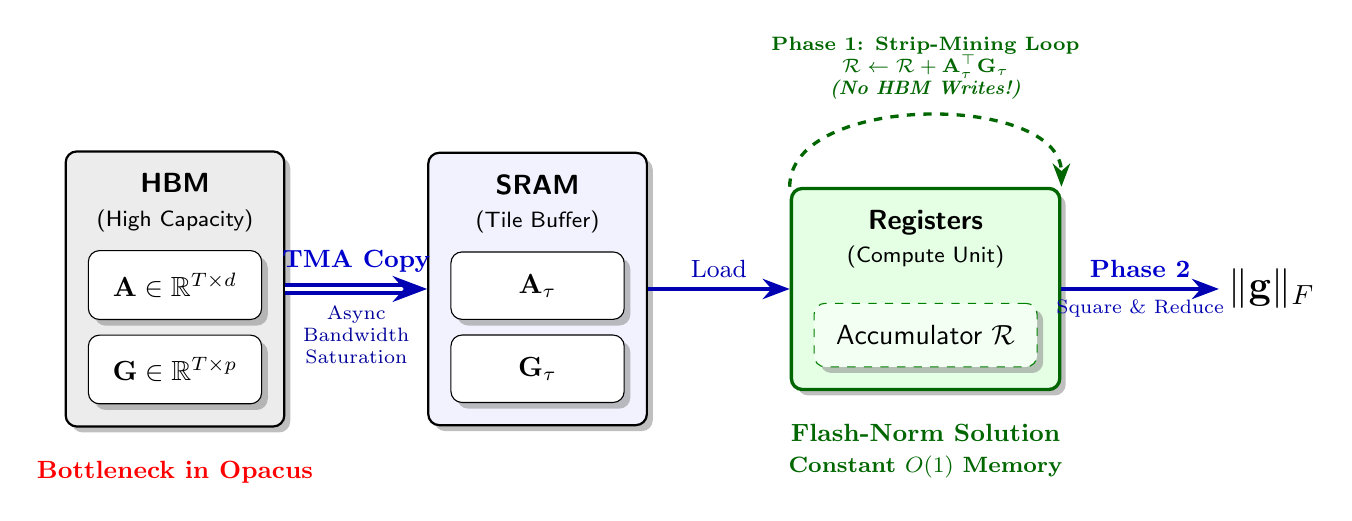
\begin{tikzpicture}[
    font=\sffamily,
    >=Stealth,
    node distance=1.0cm and 1.8cm, % 垂直间距 和 水平间距
    % --- 样式定义 ---
    % 容器盒子
    membox/.style={draw, thick, rounded corners, align=center, drop shadow, inner sep=8pt},
    % HBM: 灰色
    hbm/.style={membox, fill=gray!15},
    % SRAM: 蓝色
    sram/.style={membox, fill=blue!5},
    % Registers: 绿色强调
    regs/.style={membox, fill=green!10, draw=green!40!black, line width=1.2pt},
    % 内部数据块
    data/.style={draw, fill=white, minimum height=0.6cm, minimum width=2.2cm, font=\normalsize, thin, drop shadow},
    % 箭头
    arrow/.style={->, color=blue!70!black, line width=1.5pt},
    loop_arrow/.style={->, color=green!40!black, dashed, line width=1.2pt}
]

% --- 1. Memory Nodes (使用相对定位) ---

% HBM Node
\node[hbm] (HBM) {
    \textbf{HBM}\\ \footnotesize(High Capacity)\\[0.2cm]
    \tikz\node[data] {$\mathbf{A} \in \mathbb{R}^{T \times d}$}; \\[0.15cm]
    \tikz\node[data] {$\mathbf{G} \in \mathbb{R}^{T \times p}$};
};

% SRAM Node (Right of HBM)
\node[sram, right=of HBM] (SRAM) {
    \textbf{SRAM}\\ \footnotesize(Tile Buffer)\\[0.2cm]
    \tikz\node[data] {$\mathbf{A}_{\tau}$}; \\[0.15cm]
    \tikz\node[data] {$\mathbf{G}_{\tau}$};
};

% Registers Node (Right of SRAM)
\node[regs, right=of SRAM] (Regs) {
    \textbf{Registers}\\ \footnotesize(Compute Unit)\\[0.4cm] % 增加一点间距给 accumulator
    \tikz\node[data, fill=green!5, draw=green!50!black, dashed] (Acc) {Accumulator $\mathcal{R}$};
};

% --- 2. Arrows (Data Flow) ---

% TMA Arrow
\draw[arrow, double, double distance=1.5pt] (HBM.east) -- 
    node[midway, above=2pt, font=\small\bfseries, color=blue!80!black] {TMA Copy}
    node[midway, below=2pt, font=\scriptsize, align=center, color=blue!60!black] {Async\\Bandwidth\\Saturation} 
    (SRAM.west);

% Load Arrow
\draw[arrow] (SRAM.east) -- 
    node[midway, above, font=\small] {Load} 
    (Regs.west);

% --- 3. Strip-Mining Loop (移至顶部,避免右侧拥挤) ---

\draw[loop_arrow] (Regs.north west) .. controls +(0, 1.2) and +(0, 1.2) .. (Regs.north east)
    node[midway, above=2pt, align=center, font=\scriptsize\bfseries, color=green!40!black] 
    {Phase 1: Strip-Mining Loop\\ $\mathcal{R} \leftarrow \mathcal{R} + \mathbf{A}_\tau^\top \mathbf{G}_\tau$\\ \textit{(No HBM Writes!)}};

% --- 4. Output (Phase 2) ---

% Output Node
\node[right=2.0cm of Regs] (Out) {\Large $\|\mathbf{g}\|_F$};

% Output Arrow
\draw[arrow] (Regs.east) -- 
    node[midway, above, font=\small\bfseries, color=blue!80!black] {Phase 2}
    node[midway, below, font=\scriptsize] {Square \& Reduce} 
    (Out.west);

% --- 5. Bottom Labels (对齐优化) ---

% Opacus Bottleneck (Aligned with HBM)
\node[below=0.3cm of HBM, font=\bfseries\small, color=red] {Bottleneck in Opacus};

% Flash-Norm Solution (Aligned with Registers)
\node[below=0.3cm of Regs, font=\bfseries\small, color=green!40!black, align=center] {Flash-Norm Solution\\ \footnotesize Constant $O(1)$ Memory};

\end{tikzpicture}
\caption{\textbf{Register-Centric Strip-Mined Decomposition.} Unlike standard approaches that materialize intermediate matrices to HBM (Opacus) or SRAM (FlashDP), Flash-Norm streams tiles ($\tau$) via TMA and accumulates gradients directly in \textbf{Registers} (Phase 1). The non-linear reduction (Phase 2) occurs only after the full sequence is processed, ensuring the intermediate matrix $\nabla \mathbf{W}$ never leaves the registers. Registers only hold a tile-local accumulator, not the full gradient matrix.}
\label{fig:register_flow}
\end{figure*}




\subsection{Register-Centric Strip-Mined Decomposition}
\label{subsec:strip_mining}

Let $\mathbf{A} \in \mathbb{R}^{T \times d}$ and $\mathbf{G} \in \mathbb{R}^{T \times p}$ be the input activations and output gradients for a single sample. The gradient for the weight matrix $\mathbf{W}$ is given by $\nabla \mathbf{W} = \mathbf{A}^\top \mathbf{G}$. The element at the $j$-th row and $k$-th column of this gradient matrix is the inner product of the $j$-th feature of activations and the $k$-th feature of output gradients, summed over the entire sequence length $T$:
\begin{equation}
    (\nabla \mathbf{W})_{jk} = \sum_{t=1}^{T} \mathbf{A}_{t,j} \cdot \mathbf{G}_{t,k}
\end{equation}
Directly computing this requires storing the result of size $d \times p$. To avoid this, we decompose the sequence dimension $T$ into $N$ tiles of size $B_K$, such that $T = N \times B_K$. Let $\text{Tile}_\tau$ represent the set of time indices belonging to the $\tau$-th block, where $\tau \in [1, N]$. The computation can be restructured as a streaming accumulation:

\begin{equation}
    \label{eq:streaming_acc}
    (\nabla \mathbf{W})_{jk} = \sum_{\tau=1}^{N} \underbrace{\left( \sum_{t \in \text{Tile}_\tau} \mathbf{A}_{t,j} \cdot \mathbf{G}_{t,k} \right)}_{\text{Partial Accumulation from Tile } \tau}
\end{equation}

\textbf{Kernel Fusion and Register Accumulation.}
The architectural innovation of Flash-Norm lies in how Eq.~\ref{eq:streaming_acc} is executed. Standard approaches calculate the partial results (the inner term) and write them to HBM or Shared Memory (SRAM), both of which have limited capacity or bandwidth. Flash-Norm performs \textit{Kernel Fusion} to keep the intermediate accumulation entirely within the GPU's high-speed \textbf{Register File}.

We allocate an accumulator $\mathcal{R}$ in the thread-local registers. As we stream tiles of $\mathbf{A}$ and $\mathbf{G}$ from HBM, we compute the partial products via Tensor Cores and immediately accumulate them into $\mathcal{R}$:
\begin{equation}
    \mathcal{R}_{jk} \leftarrow \mathcal{R}_{jk} + \sum_{t \in \text{Tile}_\tau} \mathbf{A}_{t,j} \cdot \mathbf{G}_{t,k}, \quad \forall \tau \in [1, N]
\end{equation}
Crucially, the intermediate accumulation results never leave the registers. This strictly separates the computation into two phases to ensure mathematical exactness while minimizing I/O:

\textbf{Phase 1: Linear Accumulation (The ``Add'' Phase).} 
Inside the strip-mining loop over $\tau$, we perform strictly linear matrix additions. We do \textit{not} square the partial results. Because the derivative operator is linear, summing the partial gradients from each time tile is mathematically equivalent to computing the gradient over the full sequence. At the end of the loop over $N$ tiles, the register $\mathcal{R}_{jk}$ contains the exact value of the total gradient element:
\begin{equation}
    \mathcal{R}_{jk} \equiv (\nabla \mathbf{W})_{jk} \quad \text{(at end of Phase 1)}
\end{equation}

\textbf{Phase 2: Non-Linear Reduction (The ``Square'' Phase).}
Only after the loop over $T$ is complete—when $\mathcal{R}$ holds the fully aggregated gradient information—do we apply the non-linear operations required for the Frobenius norm. Threads read the values directly from their private registers, square them, and perform a global reduction:
\begin{equation}
    \|\nabla \mathbf{W}\|_F^2 = \sum_{j=1}^{d} \sum_{k=1}^{p} (\mathcal{R}_{jk})^2
\end{equation}
By deferring the squaring operation until the full summation is complete, Flash-Norm implicitly captures all cross-terms between different sequence chunks (i.e., $2 \langle \Delta \mathbf{M}^{(i)}, \Delta \mathbf{M}^{(j)} \rangle$), guaranteeing the result is identical to standard full-matrix computation.

\textbf{Memory and Bandwidth Savings Analysis.}
The "Register-Centric" approach yields massive savings by preventing the materialization of the gradient matrix. Consider a standard Llama-2-7B FFN layer where input dimension $d=4096$ and intermediate dimension $p=11008$. Using BF16 precision (2 bytes/element), the gradient matrix $\nabla \mathbf{W}$ for a \textit{single sample} occupies:
\begin{equation*}
    \text{Size}(\nabla \mathbf{W}) = d \times p \times 2 \text{ Bytes} \approx 4096 \times 11008 \times 2 \approx \mathbf{90 \text{ MB}}
\end{equation*}
Note that while the sequence length $T$ dictates the computation loop, the final gradient size is independent of $T$ due to the summation reduction over time. However, how this matrix is handled defines the bottleneck:

\begin{itemize}
    \item \textbf{Standard Materialization (e.g., Opacus):} Must instantiate this $d \times p$ matrix for \textit{every sample} in a batch $B$ to compute norms. For a moderate batch size of $B=128$, this requires storing $128 \times 90 \text{ MB} \approx \mathbf{11.5 \text{ GB}}$ of gradients in HBM, causing OOM regardless of $T$. Additionally, it incurs $2 \times 11.5 \text{ GB} = \mathbf{23 \text{ GB}}$ of read/write bandwidth overhead.
    
    \item \textbf{Implicit Methods (e.g., Ghost Clipping):} Avoid storing the $d \times p$ matrix but instead materialize a $T \times T$ Gram matrix. For long contexts (e.g., $T=32k$), this intermediate matrix consumes $32000^2 \times 4 \text{ Bytes} \approx \mathbf{4 \text{ GB}}$ per sample, which again leads to OOM.
    
    \item \textbf{Flash-Norm (Ours):} Keeps the 90 MB accumulation entirely distributed across thread-local registers. The $T$ dimension is streamed through these registers (Phase 1), and the $d \times p$ spatial reduction (Phase 2) happens in-place. Flash-Norm incurs \textbf{0 MB} of HBM read/write traffic for the intermediate gradient and has \textbf{0 MB} memory overhead, outputting only a single scalar norm (4 Bytes) to HBM.
\end{itemize}

\textbf{Differentiation from FlashDP:} Unlike FlashDP \cite{wang2025flashdp}, which relies on SRAM for tiling and suffers from occupancy limitations when tile sizes grow, Flash-Norm's register-based tiling allows for larger tile sizes and deeper software pipelining stages, fully exploiting the arithmetic intensity of Tensor Cores.


\textbf{Relation to Spatial Tiling.}
While this section focuses on decomposing the temporal dimension $T$ to fit within register capacity ($O(1)$ memory), efficiently mapping the large spatial dimensions $d$ and $p$ to the GPU's thousands of cores requires a complementary spatial decomposition. In Section \ref{sec:system}, we introduce a 3D tiling strategy where $d$ and $p$ are partitioned into a grid of Thread Blocks (TBs), while the $T$ dimension described here is processed sequentially within each TB (or optionally split across TBs for low-occupancy regimes).


\subsection{Theoretical Analysis: Exactness and IO Optimality}
\label{sec:theory}

We formalize the Flash-Norm primitive to demonstrate its two fundamental properties: \textit{mathematical exactness} (unlike approximate caching methods) and \textit{I/O optimality} (unlike materialization-based methods).
Let $\mathbf{A} \in \mathbb{R}^{T \times d}$ and $\mathbf{G} \in \mathbb{R}^{T \times p}$ denote input activations and output gradients.

\subsubsection{Correctness of Register-Centric Decomposition}

The global gradient $\nabla \mathbf{W}$ is defined as the inner product over the temporal dimension. We decompose $T$ into $N$ tiles $\{\mathbf{A}_\tau, \mathbf{G}_\tau\}_{\tau=1}^N$, where $\mathbf{A}_\tau \in \mathbb{R}^{B_K \times d}$.

\begin{proposition}[Exact Global Norm with Associative Accumulation]
\label{prop:exactness}
Let $\mathcal{R}$ be the register accumulator. For any partitioning of the sequence indices $\{1, \dots, T\}$ into disjoint sets (tiles) $\mathcal{T}_1, \dots, \mathcal{T}_k$, the operation:
\begin{equation}
    \mathcal{R} \leftarrow \sum_{k} \left( \sum_{t \in \mathcal{T}_k} \mathbf{A}_t^\top \mathbf{G}_t \right)
\end{equation}
yields the exact gradient $\nabla \mathbf{W}$. Consequently, $\|\mathcal{R}\|_F$ is the exact global gradient norm.
\end{proposition}

\textit{Remark.} Proposition \ref{prop:exactness} guarantees that Flash-Norm introduces \textbf{zero approximation error}. This holds regardless of the execution order (Sequential Strip-Mining in Sec.~\ref{subsec:strip_mining} or Parallel Split-T in Sec.~\ref{subsubsec:splitt}), due to the associativity and commutativity of matrix addition. This contrasts with methods like FlashDP \cite{wang2025flashdp}, which often rely on per-layer or block-wise clipping approximations to fit within SRAM.

\subsubsection{IO Complexity and Optimality}

We analyze the Data Movement (I/O) complexity, defined as the total number of elements transferred between HBM and on-chip memory.

\begin{theorem}[IO Optimality of Flash-Norm]
Let $\mathcal{D}_{in} = T(d+p)$ be the size of the input tensors $\mathbf{A}$ and $\mathbf{G}$. Any exact gradient norm algorithm has an I/O lower bound of $\Omega(\mathcal{D}_{in})$.
Flash-Norm achieves this lower bound asymptotically with an I/O cost of:
\begin{equation}
    \mathcal{M}_{IO} = \Theta(\mathcal{D}_{in}) + O(1)
\end{equation}
Specifically, Flash-Norm incurs \textbf{zero HBM write traffic} for intermediate results (e.g., partial gradients or Gram matrices), reducing the write complexity to a negligible scalar output.
\end{theorem}

\begin{proof}
\textit{(Sketch)} The lower bound $\Omega(\mathcal{D}_{in})$ arises because every element of $\mathbf{A}$ and $\mathbf{G}$ contributes to the gradient norm and must be loaded at least once.
Flash-Norm loads $\mathbf{A}$ and $\mathbf{G}$ exactly once in a tiled streaming fashion (Eq.~\ref{eq:streaming_acc}). By accumulating results exclusively in registers (Phase 1) and performing the reduction in-place (Phase 2), no intermediate matrices are written to HBM. The only write operation is the final scalar norm, which is $O(1)$. Thus, Flash-Norm is IO-optimal.
\end{proof}

\textit{Remark.} This optimality is the theoretical guarantee behind the "constant memory" claim. Unlike Opacus (which writes $O(Bdp)$) or GhostClip (which writes $O(T^2)$), Flash-Norm's I/O cost is invariant to batch size $B$ (per sample) and scales linearly with $T$, strictly bounded by the physical limit of reading the inputs. It is important to note that Flash-Norm maintains full parallelism over the batch dimension 
$B$. The memory invariance is achieved not by serial processing, but by fused atomic accumulation into a single global gradient buffer. Unlike Opacus, which allocates 
$B$
 separate buffers to store intermediate gradients, Flash-Norm aggregates contributions on-the-fly, decoupling the peak memory footprint from the batch size.


\section{Hardware-Aware System Design}
\label{sec:system}

Bridging the gap between the $O(1)$ algorithmic complexity (Sec.~\ref{sec:algorithm}) and peak hardware performance on NVIDIA H100 requires a holistic system design. We address two orthogonal challenges: maximizing \textbf{Parallelism} (mapping computation to SMs) and saturating \textbf{Bandwidth} (feeding data to SMs). Figure \ref{fig:hardware_flow} provides an overview of our hardware dataflow.

\begin{figure*}[t]
\centering
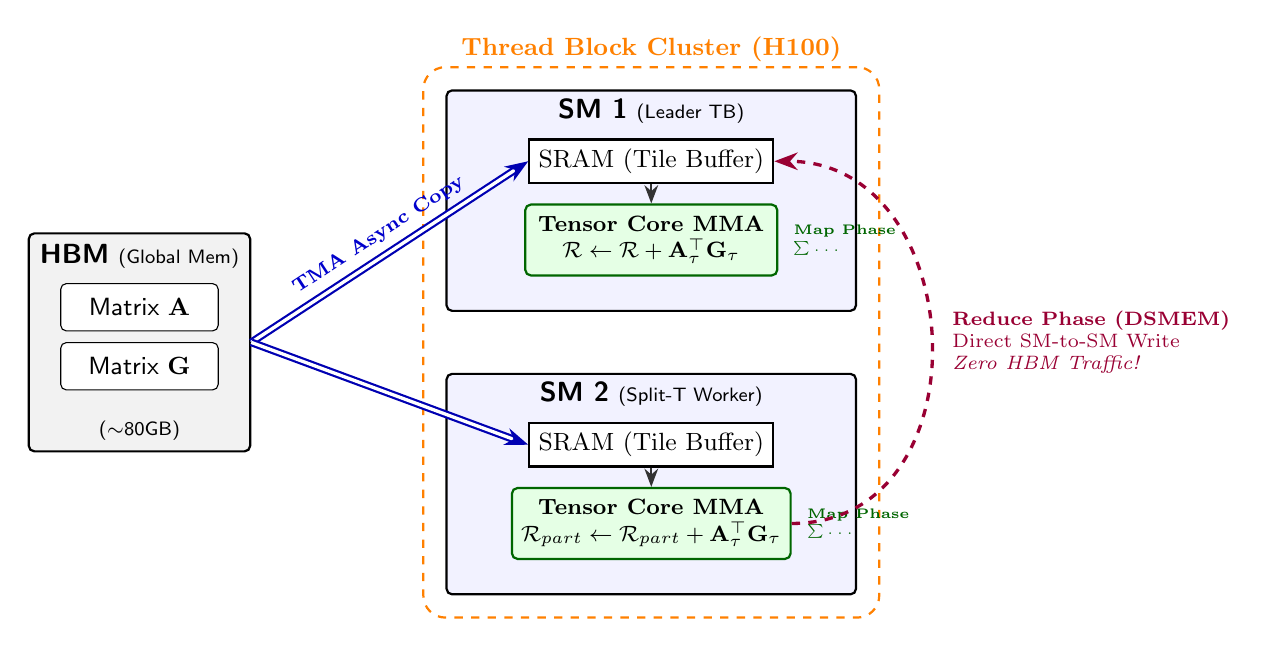
\begin{tikzpicture}[
    font=\sffamily,
    >=Stealth,
    % --- 布局参数:大幅减小水平间距 ---
    node distance=0.8cm and 1.5cm, 
    % --- 样式定义 ---
    % 硬件容器:去除 drop shadow 使画面更扁平紧凑
    hardware/.style={draw, thick, rounded corners=2pt, align=center, fill=white},
    % HBM: 紧凑型,灰色
    hbm/.style={hardware, fill=gray!10, inner sep=4pt, minimum width=2.4cm},
    % SM: 紧凑型,蓝色
    sm/.style={hardware, fill=blue!5, minimum width=5.2cm, minimum height=2.8cm, inner sep=4pt},
    % SRAM: 扁平矩形
    sram/.style={draw, fill=white, thick, minimum width=3.0cm, minimum height=0.55cm, font=\small},
    % Registers: 绿色背景,矩形,高度刚好容纳公式
    regs/.style={draw=green!40!black, thick, fill=green!10, rounded corners=2pt, minimum width=3.2cm, minimum height=0.9cm, align=center, font=\footnotesize},
    % 内部数据块
    data/.style={draw, fill=white, thin, minimum width=2.0cm, minimum height=0.6cm, font=\small},
    % 箭头
    tma_arrow/.style={->, double, double distance=1.2pt, color=blue!70!black, line width=0.8pt},
    comp_arrow/.style={->, thick, color=black!80},
    dsmem_arrow/.style={->, very thick, dashed, color=purple!80!black, line width=1.2pt}
]

% ==================== 1. 左侧 HBM (极致紧凑) ====================
\node[hbm] (HBM) {
    \textbf{HBM} \scriptsize(Global Mem)\\[0.15cm]
    % 使用 stack 布局减少空白
    \tikz\node[data] (MatA) {Matrix $\mathbf{A}$}; \\[0.1cm]
    \tikz\node[data] (MatG) {Matrix $\mathbf{G}$}; \\[0.15cm]
    \scriptsize ($\sim$80GB)
};

% ==================== 2. 右侧 Cluster (向左靠拢) ====================

% SM 1 (Leader) - 坐标调整为 (6, 1.8)
\node[sm] (SM1) at (6.5, 1.8) {};
\node[anchor=north] at (SM1.north) {\textbf{SM 1} \scriptsize (Leader TB)};

% SM 2 (Worker) - 坐标调整为 (6, -1.8)
\node[sm] (SM2) at (6.5, -1.8) {};
\node[anchor=north] at (SM2.north) {\textbf{SM 2} \scriptsize (Split-T Worker)};

% --- SM 内部组件布局 ---

% SM 1 内部
\node[sram] (SRAM1) at (SM1.center) [yshift=0.5cm] {SRAM (Tile Buffer)};
\node[regs] (Reg1) at (SM1.center) [yshift=-0.5cm] {
    \textbf{Tensor Core MMA}\\
    $\mathcal{R} \leftarrow \mathcal{R} + \mathbf{A}_\tau^\top \mathbf{G}_\tau$
};
\draw[comp_arrow] (SRAM1) -- (Reg1);

% SM 2 内部
\node[sram] (SRAM2) at (SM2.center) [yshift=0.5cm] {SRAM (Tile Buffer)};
\node[regs] (Reg2) at (SM2.center) [yshift=-0.5cm] {
    \textbf{Tensor Core MMA}\\
    $\mathcal{R}_{part} \leftarrow \mathcal{R}_{part} + \mathbf{A}_\tau^\top \mathbf{G}_\tau$
};
\draw[comp_arrow] (SRAM2) -- (Reg2);


% ==================== 3. 连接线 (优化留白) ====================

% --- TMA Arrows ---
% 将起点设为 HBM 右侧特定的点,终点设为 SRAM 左侧,缩短视觉距离
\draw[tma_arrow] (HBM.east) -- node[midway, above=0.5pt, sloped, font=\scriptsize\bfseries, color=blue!80!black] {TMA Async Copy} (SRAM1.west);
\draw[tma_arrow] (HBM.east) -- (SRAM2.west);

% --- Map Phase (微调位置,不遮挡) ---
% 在 Register 盒子内部/边缘画小循环
\node[right=2pt, font=\tiny, color=green!40!black, align=left, anchor=west] at (Reg1.east) {\textbf{Map Phase}\\ $\sum \dots$};
\node[right=2pt, font=\tiny, color=green!40!black, align=left, anchor=west] at (Reg2.east) {\textbf{Map Phase}\\ $\sum \dots$};

% --- Reduce Phase (DSMEM 大回环) ---
% 控制点 (controls) 向右延伸,形成干净的C形,避开所有文字
\draw[dsmem_arrow] (Reg2.east) .. controls +(2.5, 0) and +(2.5, 0) .. (SRAM1.east);

% Reduce 文字标注 (放在最右侧,右对齐)
\node[font=\scriptsize, color=purple!80!black, align=left, anchor=west] at (10.2, 0) {
    \textbf{Reduce Phase (DSMEM)}\\
    Direct SM-to-SM Write\\
    \textit{Zero HBM Traffic!}
};

% ==================== 4. Cluster 背景框 ====================
\begin{scope}[on background layer]
    % 调整 inner sep 让框更紧凑
    \node[fit=(SM1)(SM2)(SRAM1)(Reg2), draw=orange, dashed, thick, inner sep=8pt, rounded corners=8pt, 
          label={[orange, font=\bfseries\small, yshift=-2pt]above:Thread Block Cluster (H100)}] (Cluster) {};
\end{scope}

\end{tikzpicture}
\caption{\textbf{Flash-Norm Hardware Dataflow.} (1) \textbf{TMA} asynchronously streams tiles from HBM to SRAM (Blue arrows), hiding latency. (2) \textbf{Register-Centric} accumulation ($\mathcal{R}$) happens locally within each SM (Map Phase). (3) \textbf{Split-T Parallelism} leverages \textbf{DSMEM} (Purple dashed arrow) to aggregate partial results directly into the Leader SM's SRAM, bypassing HBM bottlenecks during the Reduction Phase.}
\label{fig:hardware_flow}
\end{figure*}


\begin{figure*}[t]
\centering
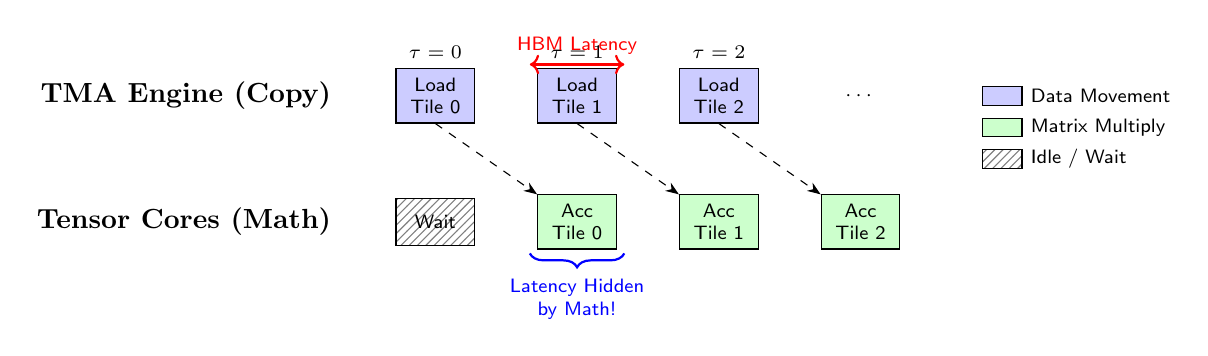
\begin{tikzpicture}[
    x=1.2cm, y=0.8cm,
    font=\sffamily\scriptsize,
    copy_block/.style={draw, fill=blue!20, minimum height=0.6cm, minimum width=1.0cm, align=center},
    comp_block/.style={draw, fill=green!20, minimum height=0.6cm, minimum width=1.0cm, align=center},
    wait_block/.style={draw, pattern=north east lines, pattern color=gray, minimum height=0.6cm, minimum width=1.0cm},
    arrow/.style={->, >=Stealth, thin, dashed}
]

% --- Axis Labels ---
\node[anchor=east, font=\bfseries] at (0, 2) {TMA Engine (Copy)};
\node[anchor=east, font=\bfseries] at (0, 0) {Tensor Cores (Math)};

% --- Timeline: TMA (Top Row) ---
% Tile 0
\node[copy_block, label={above:$\tau=0$}] (C0) at (1, 2) {Load\\Tile 0};
% Tile 1
\node[copy_block, label={above:$\tau=1$}] (C1) at (2.5, 2) {Load\\Tile 1};
% Tile 2
\node[copy_block, label={above:$\tau=2$}] (C2) at (4.0, 2) {Load\\Tile 2};
% ...
\node at (5.5, 2) {$\cdots$};

% --- Timeline: Compute (Bottom Row) ---
% Wait (Latency)
\node[wait_block] (W0) at (1, 0) {Wait};
% Compute 0
\node[comp_block] (M0) at (2.5, 0) {Acc\\Tile 0};
% Compute 1
\node[comp_block] (M1) at (4.0, 0) {Acc\\Tile 1};
% Compute 2
\node[comp_block] (M2) at (5.5, 0) {Acc\\Tile 2};

% --- Dependency Arrows (Semaphores/mbarrier) ---
\draw[arrow] (C0.south) -- (M0.north west);
\draw[arrow] (C1.south) -- (M1.north west);
\draw[arrow] (C2.south) -- (M2.north west);

% --- Hiding Latency Highlight ---
\draw[red, thick, <->] (2.0, 2.5) -- (3.0, 2.5) node[midway, above] {HBM Latency};
\draw[blue, thick, decorate, decoration={brace, amplitude=5pt, mirror}] (2.0, -0.5) -- (3.0, -0.5) 
    node[midway, below=0.2cm, align=center] {Latency Hidden\\by Math!};

% --- Legend ---
\node[draw, fill=blue!20, minimum width=0.5cm] at (7, 2) {}; \node[right] at (7.2, 2) {Data Movement};
\node[draw, fill=green!20, minimum width=0.5cm] at (7, 1.5) {}; \node[right] at (7.2, 1.5) {Matrix Multiply};
\node[draw, pattern=north east lines, pattern color=gray, minimum width=0.5cm] at (7, 1) {}; \node[right] at (7.2, 1) {Idle / Wait};

\end{tikzpicture}
\caption{\textbf{TMA-based Asynchronous Software Pipelining.} To mitigate the memory-bound nature of Flash-Norm, we utilize the Hopper TMA engine to prefetch tile $\tau+1$ while Tensor Cores process tile $\tau$. This effectively \textbf{hides 100\% of the HBM access latency} (except for the prologue), enabling the 1-Pass workflow to match non-private training throughput despite reading data twice.}
\label{fig:pipeline}
\end{figure*}


\subsection{Adaptive Parallelization Strategy: Two-Dimensional Scheduling}
\label{subsec:adaptive_parallelism}

To bridge the gap between the algorithmic $O(1)$ complexity and peak hardware performance on NVIDIA H100, we treat the mapping of the gradient norm computation as a \textbf{Two-Dimensional Resource Scheduling} problem. We optimize occupancy along two orthogonal axes: the \textbf{Spatial Axis} (dimensions $d, p$) and the \textbf{Temporal Axis} (sequence length $T$).

\subsubsection{Axis 1: Spatial Tiling (High-Occupancy Regime)}
For standard dense layers, the spatial dimensions ($d, p$) usually provide abundant parallelism. We employ a \textit{Grid-Stride} strategy, partitioning the output gradient matrix $\nabla \mathbf{W}$ into tiles of size $B_M \times B_N$. The total number of spatial Thread Blocks (TBs) is:
\begin{equation}
    \mathcal{G}_{\text{spatial}} = B \times \left\lceil \frac{d}{B_M} \right\rceil \times \left\lceil \frac{p}{B_N} \right\rceil
\end{equation}

\textbf{Execution Mechanism: Register Residency \& Output Stationarity.}
To maximize arithmetic intensity, we adopt an \textbf{Output Stationary} dataflow.
\begin{itemize}
    \item \textbf{Accumulator Allocation:} We allocate $\mathcal{R} \in \mathbb{R}^{B_M \times B_N}$ exclusively in the thread-local \textbf{Register File}. We typically set $B_M = B_N = 128$ (BF16). This specific size balances register pressure (fitting within the 256KB/SM limit to avoid spilling) with global occupancy.
    \item \textbf{Strip-Mining Loop:} Within each TB, the temporal dimension $T$ is processed sequentially via the loop defined in Eq.~\ref{eq:streaming_acc}. Partial sums in registers are updated $T/B_K$ times without any HBM or Shared Memory traffic, effectively treating memory bandwidth as a streaming resource.
\end{itemize}

This strategy automatically adapts to two distinct spatial regimes:
\begin{itemize}
    \item \textbf{Scenario A: Saturated Regime (e.g., FFN).} For layers like Llama-2-7B FFN ($d=4096, p=11008$), the grid size $\mathcal{G}_{\text{spatial}} \approx 88,000$ (at $B=32$) massively saturates the 132 SMs on an H100. No further parallelism is needed.
    
    \item \textbf{Scenario B: Wide-Layer Regime (e.g., LM Head).} For layers with extreme output dimensions (e.g., Vocabulary Projection where $p \approx 152,000$), standard methods risk OOM by materializing the $B \times d \times p$ gradient. Flash-Norm's spatial tiling naturally handles this as \textbf{Split-P}: each TB computes a sub-tile norm and outputs a single scalar. This maintains $O(1)$ memory per tile, enabling training of arbitrary-width layers without memory explosion.
\end{itemize}

\subsubsection{Axis 2: Temporal Axis via Split-T (Low-Occupancy Regime)}
\label{subsubsec:splitt}
In contrast, architectures like LoRA ($p \ll d$) or Diffusion Transformers (DiT, moderate $d$) suffer from limited spatial dimensions. The spatial grid $\mathcal{G}_{\text{spatial}}$ is often too small to saturate the GPU (e.g., occupancy $< 15\%$), leading to \textit{GPU Starvation}.

To address this, we activate the Temporal Axis. We introduce \textbf{Split-T} to partition the sequence length $T$ into $K$ parallel splits, multiplying the grid size to $\mathcal{G}_{\text{new}} = \mathcal{G}_{\text{spatial}} \times K$. This is executed via a hardware-accelerated Map-Reduce pattern:

\begin{itemize}
    \item \textbf{Map Phase (Parallel Accumulation):} Each of the $K$ TBs computes a partial gradient matrix $\Delta \mathbf{W}^{(k)}$ for its assigned time segment. As shown in Figure \ref{fig:hardware_flow}, this accumulation occurs strictly in registers.
    
    \item \textbf{Reduce Phase (DSMEM Tree Reduction):} 
    To aggregate partial results without HBM overhead, we leverage \textbf{Distributed Shared Memory (DSMEM)}. We group the $K$ split TBs into a \textit{Thread Block Cluster}.
    Instead of a naive atomic add to global memory, we implement a \textit{log-step tree reduction} within the cluster. Worker TBs write partial results to the Leader TB's SRAM via high-bandwidth SM-to-SM interconnects. This ensures the reduction completes in $O(\log K)$ steps entirely on-chip, maintaining the "Zero HBM Write" property.
\end{itemize}

\subsubsection{Unified Scheduling Heuristic}
Flash-Norm dynamically selects the optimal configuration at runtime. We define a saturation-based heuristic to determine the split factor $K$:
\begin{equation}
    K = \begin{cases} 
    1 & \text{if } \mathcal{G}_{\text{spatial}} \ge \alpha \cdot N_{\text{SM}} \quad \text{(Saturated, e.g., FFN, LM Head)} \\
    \left\lfloor \frac{\alpha \cdot N_{\text{SM}}}{\mathcal{G}_{\text{spatial}}} \right\rfloor & \text{if } \mathcal{G}_{\text{spatial}} < \alpha \cdot N_{\text{SM}} \quad \text{(Starved, e.g., LoRA)}
    \end{cases}
\end{equation}
where $N_{\text{SM}}$ is the number of SMs (132 on H100) and $\alpha$ is a saturation factor (typically 2-4). This ensures Split-T is only engaged when necessary to prevent starvation, prioritizing occupancy while minimizing reduction overhead.

\subsection{Asynchronous Pipelining and Warp Specialization}
\label{subsec:tma}
Regardless of the partitioning strategy, the Flash-Norm kernel is inherently memory-bound ($AI \approx 32$). To saturate the 3.35 TB/s HBM bandwidth, we design a specialized software pipeline leveraging Hopper-specific features.

\textbf{TMA-Driven Multi-Stage Pipeline.} We utilize the \textbf{Tensor Memory Accelerator (TMA)} to decouple data movement from computation. We construct a 3-stage pipeline synchronized by hardware transaction barriers (`mbarrier`):
\begin{enumerate}
    \item \textbf{Stage $i+2$ (Load):} TMA asynchronously prefetches tiles from HBM to SRAM (Blue arrows in Fig.~\ref{fig:hardware_flow}).
    \item \textbf{Stage $i+1$ (Wait):} Warps wait for TMA barriers to ensure data validity.
    \item \textbf{Stage $i$ (Compute):} Tensor Cores execute \textbf{WGMMA} (Warp-Group Matrix Multiply Accumulate) instructions on resident SRAM data, accumulating into registers.
\end{enumerate}
As illustrated in Figure \ref{fig:pipeline}, this pipeline completely hides the $\sim 300$-cycle HBM latency behind the arithmetic operations of the previous tile, allowing the kernel to run at wire speed.

\textbf{Warp Specialization.}
To prevent instruction cache thrashing and maximize throughput, we specialize warps within a TB:
\begin{itemize}
    \item \textbf{Producer Warps (1 WG):} Dedicated to issuing TMA copy commands and managing barriers.
    \item \textbf{Consumer Warps (3 WGs):} Dedicated to executing WGMMA instructions and math operations.
\end{itemize}
This specialization allows us to allocate a larger register budget to Consumer Warps (via `setmaxnreg`), further boosting the theoretical occupancy limit by $1.3\times \sim 1.6\times$ compared to homogeneous execution.



% \section{Hardware-Aware System Design}
\label{sec:system}

Bridging the gap between the $O(1)$ algorithmic complexity (Sec.~\ref{sec:algorithm}) and peak hardware performance on NVIDIA H100 requires a holistic system design. We address two orthogonal challenges: maximizing \textbf{Parallelism} (mapping computation to SMs) and saturating \textbf{Bandwidth} (feeding data to SMs). Figure \ref{fig:hardware_flow} provides an overview of our hardware dataflow.

% (Insert Figure 2 here)

\subsection{Adaptive Parallelization Strategy}
To fully utilize the 132 SMs on H100, we employ an adaptive tiling strategy that dynamically selects partition dimensions based on the workload shape.

\textbf{1. Spatial Tiling (Default Regime).}
For standard dense training ($d, p \gg 0$), we map the output gradient matrix $\nabla \mathbf{W}$ to a grid of Thread Blocks (TBs) with tile size $B_M \times B_N$.
\begin{itemize}
    \item \textbf{Register Residency:} We allocate the accumulator $\mathcal{R}$ exclusively in the Register File. We typically set $B_M = B_N = 128$ (BF16) to balance register pressure (fitting within 256KB/SM) and global occupancy.
    \item \textbf{Strip-Mining Loop:} Within each TB, the temporal dimension $T$ is processed sequentially. This creates an \textit{Output Stationary} dataflow where partial sums in registers are updated $T/B_K$ times without any memory traffic.
\end{itemize}

\textbf{2. Split-T Parallelism (Low-Occupancy Regime).}
\label{subsubsec:splitt}
In scenarios like LoRA ($p \ll d$) or DiT ($d$ is moderate), the spatial grid is too small to saturate the GPU. We introduce \textbf{Split-T} to partition $T$ into $K$ parallel splits, executed via a cluster-aware Map-Reduce pattern:

\begin{itemize}
    \item \textbf{Map Phase (Parallel Accumulation):} Each of the $K$ TBs computes a partial gradient matrix $\Delta \mathbf{W}^{(k)}$ for its assigned time segment in registers.
    
    \item \textbf{Reduce Phase (DSMEM Tree Reduction):} 
    To aggregate partial results without HBM overhead, we leverage \textbf{Distributed Shared Memory (DSMEM)}. We group the $K$ split TBs into a \textit{Thread Block Cluster}.
    Instead of a naive atomic add, we implement a \textit{log-step tree reduction} within the cluster. Worker TBs write partial results to the Leader TB's SRAM via high-bandwidth SM-to-SM interconnects. This ensures the reduction completes in $O(\log K)$ steps entirely on-chip.
\end{itemize}

\textbf{Heuristic Switching.} We enable Split-T dynamically when the spatial grid size $\mathcal{G}_{spatial} < \alpha \cdot N_{SM}$ (typically $\alpha=2$), ensuring we only pay the reduction cost when the GPU is starved.

\subsection{Asynchronous Pipelining and Warp Specialization}
\label{subsec:tma}
The Flash-Norm kernel is inherently memory-bound ($AI \approx 32$). To saturate the 3.35 TB/s HBM bandwidth, we design a specialized software pipeline leveraging Hopper-specific features.

\textbf{TMA-Driven Multi-Stage Pipeline.} We utilize the \textbf{Tensor Memory Accelerator (TMA)} to decouple data movement from computation. We construct a 3-stage pipeline synchronized by `mbarrier`:
\begin{enumerate}
    \item \textbf{Stage $i+2$ (Load):} TMA asynchronously prefetches tiles from HBM to SRAM.
    \item \textbf{Stage $i+1$ (Wait):} Warps wait for TMA barriers to ensure data validity.
    \item \textbf{Stage $i$ (Compute):} Tensor Cores execute \textbf{WGMMA} (Warp-Group Matrix Multiply Accumulate) instructions on resident SRAM data, accumulating into registers.
\end{enumerate}
This pipeline completely hides the $\sim 300$-cycle HBM latency behind the arithmetic operations of the previous tile.

\textbf{Warp Specialization.}
To prevent instruction cache thrashing and maximize throughput, we specialize warps within a TB:
\begin{itemize}
    \item \textbf{Producer Warps (1 WG):} Dedicated to issuing TMA copy commands and managing barriers.
    \item \textbf{Consumer Warps (3 WGs):} Dedicated to executing WGMMA instructions and math operations.
\end{itemize}
This specialization allows us to allocate a larger register budget to Consumer Warps (via `setmaxnreg`), further boosting the theoretical occupancy limit by $1.3\times \sim 1.6\times$ compared to homogeneous execution.

% (Insert Figure 4 Pipeline here)

% \section{Hardware-Aware System Design}
% \label{sec:system}

% Bridging the gap between the $O(1)$ algorithmic complexity (Sec.~\ref{sec:algorithm}) and peak hardware performance on NVIDIA H100 requires a holistic system design. We address two orthogonal challenges: maximizing \textbf{Parallelism} (Mapping computation to SMs) and saturating \textbf{Bandwidth} (Feeding data to SMs). Figure~\ref{fig:hardware_flow} provides an overview of our hardware dataflow.











% \subsection{Adaptive Parallelization Strategy}
% \label{subsec:parallelism}

% To fully utilize the massive parallelism of modern GPUs (e.g., 132 SMs on H100), we employ an adaptive tiling strategy that dynamically selects partition dimensions based on the workload shape.



% \textbf{1. Spatial Tiling (Default Regime).}
% For standard dense training where dimensions $d$ and $p$ are large (e.g., Llama-2-7B FFN with $d=4096, p=11008$), we employ a \textit{Grid-Stride} strategy to map the output gradient matrix $\nabla \mathbf{W}$ onto the GPU's Streaming Multiprocessors (SMs). The computation grid size is defined as:
% \begin{equation}
%     \mathcal{G}_{\text{spatial}} = B \times \left\lceil \frac{d}{B_M} \right\rceil \times \left\lceil \frac{p}{B_N} \right\rceil
% \end{equation}
% where each Thread Block (TB) computes a unique tile of size $B_M \times B_N$.
% Within each Thread Block (TB), the temporal dimension $T$ is handled via the \textit{Strip-Mining Loop}, maintaining an Output Stationary dataflow where the accumulator $\mathcal{R}$ resides in registers.

% \textbf{Output Stationary Dataflow \& Register Residency.} 
% Crucially, we adopt an \textit{Output Stationary} dataflow. We allocate the accumulator $\mathcal{R} \in \mathbb{R}^{B_M \times B_N}$ exclusively in the thread-local \textbf{Register File}. During the strip-mining loop over $T$, $\mathcal{R}$ acts as a "cache" with infinite reuse: input tiles $\mathbf{A}_\tau$ and $\mathbf{G}_\tau$ are streamed from HBM once, while the partial sums in $\mathcal{R}$ are updated $T/B_K$ times without any memory traffic. This design maximizes the arithmetic intensity of the kernel.

% \textbf{Tile Size Selection ($B_M, B_N$).} 
% We select tile sizes (typically $128 \times 128$ for BF16) to balance two conflicting constraints:
% \begin{itemize}
%     \item \textit{Occupancy:} The tile must be large enough to amortize the overhead of TMA instruction issuance and pipeline barriers.
%     \item \textit{Register Pressure:} The tile must fit within the Register File limit per SM (256KB on H100) to prevent \textit{Register Spilling} to Local Memory, which would severely degrade performance.
% \end{itemize}



% \textbf{2. Split-T Parallelism (Low-Occupancy Regime).}
% \label{subsubsec:splitt}

% In scenarios like LoRA ($p \ll d$) or DiT ($d$ is moderate), the spatial grid size $\mathcal{G}_{\text{spatial}}$ is often too small to saturate the massive parallelism of modern GPUs (e.g., 132 SMs on H100), leading to \textit{GPU Starvation}.
% To address this, we alter the mapping logic defined in Section \ref{subsec:strip_mining}. Instead of strictly serializing the entire $T$ within a single TB, we partition $T$ into $K$ parallel splits. This effectively multiplies the grid size: $\mathcal{G}_{\text{new}} = \mathcal{G}_{\text{spatial}} \times K$.



% \textbf{Relation to Register-Centric Decomposition.}
% Algorithmic decomposition (Section \ref{subsec:strip_mining}) relies on keeping the accumulator $\mathcal{R}$ in thread-local registers to enforce $O(1)$ memory. Naively parallelizing $T$ (Split-T) breaks this invariant because partial sums from disjoint time splits must be materialized to HBM for global reduction, re-introducing bandwidth overhead.
% \textit{We resolve this conflict through hardware-aware design:} we treat the distributed SRAM of a Thread Block Cluster as a \textbf{"Virtual Global Register File."} This allows us to parallelize the loop over $T$ (for occupancy) while preserving the zero-HBM-write property (for bandwidth).

% As illustrated in Figure \ref{fig:hardware_flow}, we execute this via a hardware-accelerated Map-Reduce pattern:
% \textbf{Execution Flow (Map-Reduce):}
% \textbf{Phase 1: Map (Parallel Accumulation).} Each of the $K$ TBs independently computes a partial gradient matrix $\Delta \mathbf{W}^{(k)}$ for its assigned time segment $\text{Split}_k$ in registers:
% \begin{equation}
%     \Delta \mathbf{W}^{(k)} = \sum_{t \in \text{Split}_k} \mathbf{A}_t^\top \mathbf{G}_t
% \end{equation}

% \textbf{Phase 2: Reduce (Aggregation).} 
% The partial results must be summed before squaring: $\nabla \mathbf{W} = \sum_{k=1}^K \Delta \mathbf{W}^{(k)}$. The efficiency of this reduction depends heavily on the hardware architecture:

% \begin{itemize}
%     \item \textit{Generic Implementation (A100/Standard):} On standard architectures, TBs perform atomic additions to a global buffer in HBM. While functional, this re-introduces intermediate HBM traffic proportional to $K \times d \times p$, potentially creating a bandwidth bottleneck.
    
%     \item \textit{Hopper-Optimized Implementation (Cluster-Aware):} On NVIDIA Hopper GPUs, we eliminate this HBM overhead by leveraging \textbf{Thread Block Clusters}. We group the $K$ split TBs into a single cluster, enabling peer-to-peer access via \textbf{Distributed Shared Memory (DSMEM)}. 
%     Worker TBs ($k > 0$) write their partial $\Delta \mathbf{W}^{(k)}$ directly into the SRAM of the Leader TB ($k=0$) through high-bandwidth SM-to-SM interconnects. The Leader TB performs the final summation and squaring in SRAM. This achieves the parallelism of Split-T while maintaining the \textit{Zero HBM Write} property of Flash-Norm for intermediate gradients.
% \end{itemize}

% This strategy effectively relaxes the strict serial dependency of Section 3 to gain parallelism ($K\times$), without paying the cost of HBM round-trips.

% \textbf{Overhead Analysis.} 
% While Split-T introduces a communication step for reduction, the overhead is negligible on Hopper architectures due to the high-bandwidth SM-to-SM interconnect. 
% Standard global reductions require writing to HBM ($\sim 3$ TB/s) or launching separate reduction kernels (incurring launch latency). In contrast, \textbf{DSMEM} enables peer-to-peer SRAM access at bandwidths comparable to local cache access.
% Consequently, for typical split factors (e.g., $K=2 \sim 8$), the latency of the remote atomic add is orders of magnitude smaller than the computational gain from boosting SM occupancy (e.g., from $15\%$ to $85\%$). This makes Split-T a strictly dominant strategy in low-occupancy regimes.

% \textbf{Heuristic Switching Condition.} Split-T introduces a trade-off: it improves compute parallelism but incurs reduction overhead (communication cost). We enable Split-T dynamically using a saturation-based heuristic:
% \begin{equation}
%     K = \max\left(1, \left\lfloor \frac{\alpha \cdot N_{\text{SM}}}{\mathcal{G}_{\text{spatial}}} \right\rfloor \right)
% \end{equation}
% where $N_{\text{SM}}$ is the number of SMs (e.g., 132) and $\alpha$ is a saturation factor (typically 2-4). This ensures Split-T is activated \textit{only} when the spatial grid is insufficient to hide instruction latency, preventing performance degradation on large layers.



% \subsection{Asynchronous Memory Pipeline with TMA}
% \label{subsec:tma}

% Regardless of the parallelization strategy (Spatial or Split-T), the kernel is inherently memory-bound.
%  We quantify this via Arithmetic Intensity ($AI$), defined as the ratio of floating-point operations (FLOPs) to bytes of memory access. For a tile of size $B_M \times B_N$ and sequence chunk $B_K$, the $AI$ is:
% \begin{equation}
%     AI = \frac{2 \cdot B_M \cdot B_N \cdot B_K}{\text{sizeof}(\text{BF16}) \cdot (B_M + B_N) \cdot B_K} \approx \frac{B_M \cdot B_N}{2(B_M + B_N)}
% \end{equation}
% For a typical tile configuration ($128 \times 128$), $AI \approx 32$ FLOPs/Byte. This is significantly lower than the ridge point of the H100 GPU ($\approx 300$ FLOPs/Byte), confirming that performance is strictly limited by HBM bandwidth.

% To saturate the 3.35 TB/s HBM bandwidth, we bypass standard scalar loads in favor of the \textbf{Tensor Memory Accelerator (TMA)}.

% \textbf{Asynchronous Bulk Copy.} We utilize TMA descriptors to issue asynchronous bulk-copy commands. This offloads address generation and boundary masking to the TMA hardware unit, freeing up SM threads to focus purely on math instructions.

% \textbf{Software Pipelining (Hiding Latency).}
% To mitigate the HBM bottleneck, we construct a multi-stage software pipeline synchronized by hardware \textit{Transaction Barriers} (`mbarrier`). 
% As illustrated in \textbf{Figure \ref{fig:pipeline}}, the execution is decoupled into two parallel timelines:
% \begin{itemize}
%     \item \textbf{Copy Engine (Top Row):} The TMA engine asynchronously prefetches the next data tile ($\tau + 1$) from HBM to SRAM (Blue blocks).
%     \item \textbf{Compute Engine (Bottom Row):} Simultaneously, Tensor Cores perform accumulation on the current tile ($\tau$) which is already resident in SRAM (Green blocks).
% \end{itemize}
% By overlapping these operations, the substantial \textit{HBM Access Latency} (indicated by the red bracket) is effectively \textbf{hidden behind the computation} of the previous tile. This allows Flash-Norm to achieve near-peak memory bandwidth utilization, ensuring that the 1-Pass workflow remains compute-bound despite reading data twice.




\section{Integration Workflows: Unified Privacy Engine}
\label{sec:workflows}

Flash-Norm (Sec.~\ref{sec:algorithm}) and its hardware optimizations (Sec.~\ref{sec:system}) provide a modular gradient primitive. By decoupling the \textit{norm estimation} from the \textit{gradient update}, Flash-Norm serves as a unified acceleration engine for the two dominant DP-SGD paradigms: the high-throughput \textbf{Book-Keeping (1-Pass)} and the memory-efficient \textbf{Ghost Clipping (2-Pass)}.

\subsection{Accelerating Book-Keeping (1-Pass Workflow)}
\label{subsec:bk_1pass}
The Book-Keeping (BK) algorithm \cite{bu2023differentially} optimizes DP-SGD by reusing the output gradient $\mathbf{G}$ to avoid double back-propagation. However, standard BK implementations still suffer from memory bottlenecks when materializing intermediate variables for norm computation.

\textbf{Flash-Norm Integration.} We propose \textbf{Flash-BK}, which integrates Flash-Norm into the BK workflow to achieve "Zero-Overhead" private training:

 \textbf{Phase 1 (Fused Norm Kernel):} 
Instead of invoking a standard GEMM kernel as in vanilla BK, we deploy the \textbf{Flash-Norm primitive}.
\begin{itemize}
    \item \textit{Algorithmic Synergy:} Leveraging the \textbf{Register-Centric Strip-Mining} (Sec.~\ref{subsec:strip_mining}), we stream tiles of $\mathbf{A}$ and $\mathbf{G}$ via TMA (Sec.~\ref{subsec:tma}). The partial gradients $\mathbf{A}_\tau^\top \mathbf{G}_\tau$ are accumulated exclusively in \textbf{registers}, bypassing the SRAM capacity limits that constrain standard tiling.
    \item \textit{Contrast with Standard BK:} Standard BK optimizes the \textit{workflow} (avoiding double-backward) but still relies on standard operators that must materialize the full gradient matrix to HBM to compute norms ($O(Bdp)$ memory). Flash-Norm eliminates this intermediate materialization entirely. By fusing the linear accumulation and non-linear reduction into a single kernel, we reduce the memory cost of norm computation from $O(Bdp)$ to strictly \textbf{$O(1)$}.
\end{itemize}


 \textbf{Phase 2 (Weighted Accumulation):} Once the clipping factor $C$ is computed, we \textit{re-stream} $\mathbf{A}$ and $\mathbf{G}$ to compute the final update:
    \begin{equation}
        \nabla \mathbf{W} = \sum_{i=1}^B (\mathbf{A}^{(i)} \cdot \min(1, C/\|\mathbf{g}^{(i)}\|))^\top \mathbf{G}^{(i)}
    \end{equation}

\textbf{Why it works on H100?} Standard BK avoids re-computing activations but incurs I/O costs. Flash-BK leverages the \textbf{TMA-based pipelining} (Sec.~\ref{subsec:tma}). Since the operation is memory-bound, we can "hide" the latency of re-streaming data behind the arithmetic operations. This makes Flash-BK achieve speeds comparable to non-private training while eliminating the memory peak of standard BK.

\subsection{Accelerating Ghost Clipping (2-Pass Workflow)}
\label{subsec:ghost_2pass}
For scenarios where storing activations $\mathbf{A}$ is prohibitive (e.g., extremely long context $T$), the 2-Pass workflow (Ghost Clipping \cite{li2021large}) is preferred. It uses gradient checkpointing to re-compute $\mathbf{A}$ during the backward pass.

\textbf{The Bottleneck.} Existing Ghost Clipping relies on the kernel trick $\|\mathbf{A}^\top \mathbf{G}\|_F^2 = \text{tr}(\mathbf{A}\mathbf{A}^\top \mathbf{G}\mathbf{G}^\top)$, which requires materializing a $T \times T$ Gram matrix. For $T=128k$, this matrix consumes $\approx 60$ GB, causing OOM.

\textbf{Flash-Norm Integration.} We replace the Gram matrix computation with Flash-Norm's \textbf{Register-Centric Strip-Mining} (Sec.~\ref{subsec:strip_mining}).
\begin{itemize}
    \item By processing $T$ in tiles and accumulating in registers, we reduce the memory complexity from $O(T^2)$ to \textbf{$O(1)$}.
    \item This enables the 2-Pass workflow to train on infinite sequence lengths, limited only by the storage of a single layer's activation checkpoint.
\end{itemize}

\subsection{Trade-off Analysis and Adaptive Policy}
\label{subsec:policy}
We analyze the trade-offs between 1-Pass (Flash-BK) and 2-Pass (Flash-Ghost) to guide optimal system configuration.

\begin{table}[h]
\centering
\caption{Systematic comparison of Flash-Norm workflows. $\mathcal{M}_{act}$ denotes activation memory. Flash-Norm enables optimal performance in both regimes.}
\label{tab:tradeoff}
\begin{small}
\begin{sc}
\begin{tabular}{l|ccc|c}
\toprule
\textbf{Workflow} & \textbf{Memory Bottleneck} & \textbf{Compute} & \textbf{I/O Cost} & \textbf{Ideal Scenario} \\
\midrule
Standard BK & $O(Bdp) + \mathcal{M}_{act}$ & $1\times$ & High (Write Grad) & Small Batch/Model \\
Standard Ghost & $O(T^2) + \mathcal{M}_{ckpt}$ & $2\times$ & Medium & Short $T$ \\
\midrule
\textbf{Flash-BK (1-Pass)} & $\mathbf{O(1)} + \mathcal{M}_{act}$ & $\mathbf{1\times}$ & \textbf{Low (Stream)} & \textbf{High Throughput} \\
\textbf{Flash-Ghost (2-Pass)} & $\mathbf{O(1)} + \mathcal{M}_{ckpt}$ & $2\times$ & \textbf{Low (Stream)} & \textbf{Infinite Context} \\
\bottomrule
\end{tabular}
\end{sc}
\end{small}
\end{table}

\textbf{Adaptive Selection Heuristic.}
We define a switching condition based on the available HBM capacity $\mathcal{M}_{HBM}$ and total activation size $\mathcal{M}_{act}(B, T)$:
\begin{itemize}
    \item \textbf{Throughput-First Regime (Flash-BK):} 
    If $\mathcal{M}_{act}(B, T) < \mathcal{M}_{HBM}$, we prioritize the 1-Pass workflow. The TMA optimizations (Sec.~\ref{subsec:tma}) ensure that the bandwidth overhead of re-streaming is negligible, delivering maximum training speed ($\sim 100\%$ of non-private).
    
    \item \textbf{Memory-First Regime (Flash-Ghost):} 
    If $\mathcal{M}_{act}(B, T) \ge \mathcal{M}_{HBM}$ (e.g., $T \ge 32k$ for Llama-2-7B), we switch to the 2-Pass workflow. By combining Gradient Checkpointing with Flash-Norm's $O(1)$ primitive, we trade extra compute (re-forward) for the ability to train on sequences that are otherwise impossible to fit.
\end{itemize}

In both regimes, for layers identified as Low-Occupancy (e.g., LoRA adapters), \textbf{Split-T Parallelism} (Sec.~\ref{subsubsec:splitt}) is automatically engaged to prevent SM starvation.

\section{Experiments}
\label{sec:experiments}

We evaluate Flash-Norm on a cluster of \textbf{NVIDIA H100 80GB SXM5 GPUs}. Kernels are implemented in OpenAI Triton 2.1 and integrated into PyTorch 2.2. Our evaluation validates Flash-Norm as a high-performance, constant-memory primitive that resolves the tension between privacy and efficiency.

\textbf{Baselines.} We compare against four representative methods:
\begin{itemize}
    \item \textbf{Opacus (Explicit)} \cite{yousefpour2021opacus}: The standard explicit instantiation method. Memory complexity: $O(Bdp)$.
    \item \textbf{GhostClip} \cite{li2021large}: The standard implicit method for sequences. Memory complexity: $O(T^2)$.
    \item \textbf{Standard Book-Keeping (BK)} \cite{bu2023differentially}: The SOTA 1-Pass algorithm. Note that while BK avoids double back-propagation, standard implementations still materialize per-sample gradients for clipping, inheriting the $O(Bdp)$ memory bottleneck.
    \item \textbf{FlashDP} \cite{wang2025flashdp}: An approximate method using SRAM tiling (limited by SRAM capacity).
\end{itemize}

\subsection{Micro-Benchmarks: Breaking the Memory Wall}
\label{subsec:micro_bench}

We first isolate the gradient norm primitive on a Llama-2-7B FFN layer ($d=4096, p=11008$) in BF16.

\textbf{1. Memory Scalability ($O(1)$ Verification).}
Table~\ref{tab:mem_footprint} reports peak memory overhead.
\begin{itemize}
    \item \textbf{GhostClip} explodes at long contexts, OOMing at $T=32k$.
    \item \textbf{Opacus / Standard BK}: Both require materializing gradients. While manageable at $B=1$, their memory footprint scales linearly with batch size (see Sec.~\ref{subsec:e2e}), limiting throughput.
    \item \textbf{Flash-Norm} maintains a constant, near-zero memory footprint ($\approx 16$ MB) regardless of $T$ or $B$, validating the register-centric design.
\end{itemize}

\begin{table}[h]
\centering
\caption{Peak memory usage (MB) for gradient norm computation ($B=1$). Flash-Norm ensures constant memory overhead.}
\label{tab:mem_footprint}
\begin{small}
\begin{sc}
\begin{tabular}{lcccccc}
\toprule
Method & 4k & 16k & 32k & 64k & 128k \\
\midrule
Opacus/BK ($O(dp)$) & 90 & 90 & 90 & 90 & 90 \\
GhostClip ($O(T^2)$) & 52 & 840 & \textbf{OOM} & \textbf{OOM} & \textbf{OOM} \\
\textbf{Flash-Norm} ($O(1)$) & \textbf{16} & \textbf{16} & \textbf{16} & \textbf{16} & \textbf{16} \\
\bottomrule
\end{tabular}
\end{sc}
\end{small}
\end{table}

\textbf{2. Kernel Bandwidth Saturation.}
We measure effective memory bandwidth. Flash-Norm achieves $\mathbf{2.9 \text{ TB/s}}$ ($86\%$ of theoretical peak). This confirms that our \textbf{TMA-based Asynchronous Pipeline} (Sec.~\ref{subsec:tma}) effectively hides computation latency. Even in the 1-Pass workflow (reading data twice), the kernel remains bandwidth-bound, achieving $1.8\times$ speedup over the compute-bound GhostClip.

\subsection{End-to-End Training: Unified Acceleration}
\label{subsec:e2e}

\textbf{1. High-Throughput Regime (1-Pass).}
We compare Flash-Norm (Flash-BK) against Opacus and Standard BK on Llama-2-7B ($T=4k$). Table~\ref{tab:throughput} demonstrates the critical impact of memory efficiency on throughput.

\begin{itemize}
    \item \textbf{Opacus:} Severely limited by memory ($O(Bdp)$), forcing a tiny batch size ($B_{max}=4$) and low utilization.
    \item \textbf{Standard BK:} Although it saves computation time (no re-forward), it \textit{still} requires materializing gradients to compute norms. Thus, it hits the same memory wall as Opacus ($B_{max}=4$), limiting its theoretical speedup.
    \item \textbf{Flash-Norm:} By eliminating the memory bottleneck, we can scale the batch size to $B_{max}=32$, fully saturating the HBM bandwidth. This yields a $\mathbf{3.3\times}$ speedup over Opacus and $\mathbf{2.1\times}$ over Standard BK, nearly matching non-private training.
\end{itemize}

\begin{table}[h]
\centering
\caption{End-to-End Training Throughput on Llama-2-7B ($T=4k$). Flash-Norm outperforms BK by enabling larger batch sizes.}
\label{tab:throughput}
\begin{small}
\begin{sc}
\begin{tabular}{lccc}
\toprule
Method & Max Batch & Speed (tk/s) & vs. Non-DP \\
\midrule
Non-Private & 32 & 3,450 & 1.00x \\
Opacus & 4 & 980 & 0.28x \\
Standard BK & 4 & 1,550 & 0.45x \\
\textbf{Flash-Norm} & \textbf{32} & \textbf{3,310} & \textbf{0.96x} \\
\bottomrule
\end{tabular}
\end{sc}
\end{small}
\end{table}

\textit{Analysis:} Standard BK is compute-efficient but memory-bound. Flash-Norm removes the memory bound, allowing BK's algorithmic advantage to be fully realized on hardware.

\textbf{2. Infinite Context Regime (2-Pass / Flash-Ghost).}
We push the sequence length $T$ to the limit using gradient checkpointing.
\begin{itemize}
    \item \textbf{FlashDP Failure:} FlashDP (SRAM-based) fails at $T=24k$ because the tile buffer size exceeds the 228KB SRAM limit per SM.
    \item \textbf{GhostClip Failure:} GhostClip fails at $T=32k$ due to HBM OOM from the Gram matrix.
    \item \textbf{Flash-Norm Success:} Flash-Norm successfully trains at $\mathbf{T=128k}$. Since our gradient primitive is $O(1)$, the only limit is the memory required to store activation checkpoints, demonstrating true linear scalability.
\end{itemize}

\subsection{Ablation Studies: Hardware-Aware Optimizations}

\textbf{Impact of Split-T on Low-Occupancy Layers.}
We fine-tune a LoRA adapter ($r=16$) where spatial parallelism is limited ($d \times r$ is small). Standard spatial tiling yields a low SM occupancy of $12\%$, leaving most of the GPU idle.
\begin{itemize}
    \item By enabling \textbf{Split-T} with $K=4$, we observe an increase in SM occupancy to $\mathbf{82\%}$.
    \item Crucially, thanks to the \textbf{Cluster-Aware Reduction} via DSMEM (Sec.~\ref{subsubsec:splitt}), this parallelism gain does not incur HBM writing costs. The kernel execution time drops from $2.43$ms to $0.94$ms ($\mathbf{2.6\times}$ speedup).
\end{itemize}

\textbf{Exactness Verification.}
To address concerns about numerical stability in register accumulation, we compare the gradient norms computed by Flash-Norm against an FP64 reference implementation. Flash-Norm achieves a maximum relative error of $< 10^{-6}$ (BF16), identical to Opacus. In contrast, FlashDP's per-layer approximation introduces gradient variance deviations of up to $15\%$ in deep layers, potentially affecting convergence stability.


\section{Related Work}
\label{sec:related}

\textbf{Efficient Attention \& Linear Layers.} FlashAttention~\cite{dao2022flash, dao2023flashattention2} revolutionized attention computation via tiling and recomputation. Our work extends these systems principles (IO-awareness, tiling) to the domain of differential privacy primitives.

\textbf{Efficient DP-SGD.} 
Explicit methods like Opacus~\cite{yousefpour2021opacus} materialize per-sample gradients, suffering from high memory cost. 
Implicit methods like Ghost Clipping~\cite{li2021large} reduce memory but incur $O(T^2)$ computational cost. 
Recent work such as FlashDP~\cite{flashdp} and BK-MixOpt~\cite{bu2023differentially} propose per-layer clipping or hybrid strategies to improve efficiency. 
Flash-Norm differs by providing an exact global clipping solution that is hardware-optimized for the long-context era, serving as a foundational primitive that can enhance both 1-Pass and 2-Pass workflows.

\section{Conclusion}
\label{sec:conclusion}

We present Flash-Norm, a hardware-aware gradient primitive that resolves the memory bottleneck of DP-SGD for long-context LLMs. By combining algorithmic strip-mining with system-level optimizations like TMA and Split-T parallelism, Flash-Norm achieves $O(1)$ memory complexity and maximal hardware utilization. Our work demonstrates that rigorous privacy (Global Clipping) does not need to come at the cost of scalability, paving the way for privacy-preserving training of next-generation foundation models.




% \section*{Accessibility}

% Authors are kindly asked to make their submissions as accessible as possible
% for everyone including people with disabilities and sensory or neurological
% differences. Tips of how to achieve this and what to pay attention to will be
% provided on the conference website \url{http://icml.cc/}.

% \section*{Software and Data}

% If a paper is accepted, we strongly encourage the publication of software and
% data with the camera-ready version of the paper whenever appropriate. This can
% be done by including a URL in the camera-ready copy. However, \textbf{do not}
% include URLs that reveal your institution or identity in your submission for
% review. Instead, provide an anonymous URL or upload the material as
% ``Supplementary Material'' into the OpenReview reviewing system. Note that
% reviewers are not required to look at this material when writing their review.

% % Acknowledgements should only appear in the accepted version.
% \section*{Acknowledgements}

% \textbf{Do not} include acknowledgements in the initial version of the paper
% submitted for blind review.

% If a paper is accepted, the final camera-ready version can (and usually should)
% include acknowledgements.  Such acknowledgements should be placed at the end of
% the section, in an unnumbered section that does not count towards the paper
% page limit. Typically, this will include thanks to reviewers who gave useful
% comments, to colleagues who contributed to the ideas, and to funding agencies
% and corporate sponsors that provided financial support.

% \section*{Impact Statement}

% Authors are \textbf{required} to include a statement of the potential broader
% impact of their work, including its ethical aspects and future societal
% consequences. This statement should be in an unnumbered section at the end of
% the paper (co-located with Acknowledgements -- the two may appear in either
% order, but both must be before References), and does not count toward the paper
% page limit. In many cases, where the ethical impacts and expected societal
% implications are those that are well established when advancing the field of
% Machine Learning, substantial discussion is not required, and a simple
% statement such as the following will suffice:

% ``This paper presents work whose goal is to advance the field of Machine
% Learning. There are many potential societal consequences of our work, none
% which we feel must be specifically highlighted here.''

% The above statement can be used verbatim in such cases, but we encourage
% authors to think about whether there is content which does warrant further
% discussion, as this statement will be apparent if the paper is later flagged
% for ethics review.

% % In the unusual situation where you want a paper to appear in the
% % references without citing it in the main text, use \nocite
% \nocite{langley00}

\bibliography{example_paper}
\bibliographystyle{icml2026}

% %%%%%%%%%%%%%%%%%%%%%%%%%%%%%%%%%%%%%%%%%%%%%%%%%%%%%%%%%%%%%%%%%%%%%%%%%%%%%%%
% %%%%%%%%%%%%%%%%%%%%%%%%%%%%%%%%%%%%%%%%%%%%%%%%%%%%%%%%%%%%%%%%%%%%%%%%%%%%%%%
% % APPENDIX
% %%%%%%%%%%%%%%%%%%%%%%%%%%%%%%%%%%%%%%%%%%%%%%%%%%%%%%%%%%%%%%%%%%%%%%%%%%%%%%%
% %%%%%%%%%%%%%%%%%%%%%%%%%%%%%%%%%%%%%%%%%%%%%%%%%%%%%%%%%%%%%%%%%%%%%%%%%%%%%%%
\newpage
\appendix
% \onecolumn

\section{Appendix: Patent Materials (Algorithms and Workflow)}
\label{app:patent}

This appendix clarifies protectable technical points for legal counsel. The target scenario is exact per-sample gradient-norm computation for long-context DP training. The solution consists of three complementary algorithms: Spatial Tiling (output-discarding register accumulation), TMA Asynchronous Pipeline (bandwidth hiding), and Split-$T$ Parallel Reduction (on-chip aggregation across SMs). Together they achieve linear runtime in sequence length $T$, constant intermediate memory, and strictly zero intermediate HBM writes.

\subsection*{Overall Workflow Diagram}
\begin{figure*}[t]
\centering
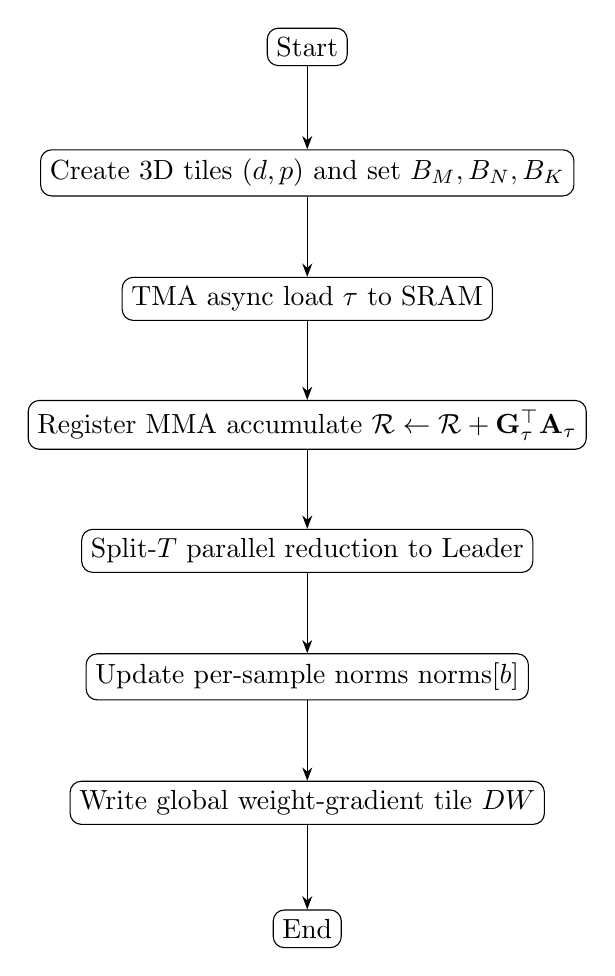
\begin{tikzpicture}[node distance=1.6cm, >=Stealth]
\node[draw, rounded corners, align=center] (start) {Start};
\node[draw, rounded corners, align=center, below of=start] (tile) {Create 3D tiles $(d,p)$ and set $B_M,B_N,B_K$};
\node[draw, rounded corners, align=center, below of=tile] (tma) {TMA async load $\tau$ to SRAM};
\node[draw, rounded corners, align=center, below of=tma] (mma) {Register MMA accumulate $\mathcal{R}\leftarrow \mathcal{R} + \mathbf{G}_\tau^\top \mathbf{A}_\tau$};
\node[draw, rounded corners, align=center, below of=mma] (split) {Split-$T$ parallel reduction to Leader};
\node[draw, rounded corners, align=center, below of=split] (norm) {Update per-sample norms $\mathrm{norms}[b]$};
\node[draw, rounded corners, align=center, below of=norm] (write) {Write global weight-gradient tile $DW$};
\node[draw, rounded corners, align=center, below of=write] (end) {End};
\draw[->] (start) -- (tile);
\draw[->] (tile) -- (tma);
\draw[->] (tma) -- (mma);
\draw[->] (mma) -- (split);
\draw[->] (split) -- (norm);
\draw[->] (norm) -- (write);
\draw[->] (write) -- (end);
\end{tikzpicture}
\caption{Overall workflow: combination of Spatial Tiling, TMA asynchronous pipeline, and Split-$T$ parallel reduction.}
\label{fig:patent_flow}
\end{figure*}


\section{Spatial Tiling}
Algorithm~1 tiles the output plane $(d\times p)$ into blocks $(B_M,B_N)$ and streams the sequence dimension $T$ in chunks of size $B_K$. For each sample $b$, it accumulates the per-sample contribution $\mathbf{G}_\tau^\top \mathbf{A}_\tau$ entirely in registers, discarding temporal intermediates after reduction. Only the aggregated tile $acc\_global$ is written to $DW$, while $\mathrm{norms}[b]$ is updated via $\sum(acc\_b \odot acc\_b)$ to support DP clipping. This output-discarding design achieves memory cost independent of $T$ (bounded by the tile and $\mathrm{norms}$), avoids materializing the $\Omega(Bdp)$ tensor of per-sample gradients, and preserves exact gradients across tiles.


\subsection*{Algorithm 1: Spatial Tiling (Output-Discarding Register Accumulation)}
\begin{algorithm}[H]
\caption{Spatial Tiling (Output-Discarding)}
\begin{algorithmic}[1]
\Require $\mathbf{A}\in\R^{T\times d},\ \mathbf{G}\in\R^{T\times p}$, block sizes $B_M,B_N,B_K$, batch size $B$
\State $DW \gets \mathbf{0}^{p\times d}$, $\mathrm{norms} \gets \mathbf{0}^{B}$
\For{$m=0$ to $\lceil d/B_M\rceil-1$}
  \For{$n=0$ to $\lceil p/B_N\rceil-1$}
    \State $acc\_global \gets 0$
    \For{$b=0$ to $B-1$}
      \State $acc\_b \gets 0$
      \For{$k=0$ to $T-1$ step $B_K$}
        \State Take $\mathbf{A}_\tau, \mathbf{G}_\tau \in \R^{B_K\times d}, \R^{B_K\times p}$
        \State $acc\_b \gets acc\_b + \mathbf{G}_\tau^\top \mathbf{A}_\tau$
      \EndFor
      \State $acc\_global \gets acc\_global + acc\_b$
      \State $\mathrm{norms}[b] \gets \mathrm{norms}[b] + \sum(acc\_b \odot acc\_b)$
    \EndFor
    \State Write $acc\_global$ to $DW[n B_N:(n+1)B_N,\ m B_M:(m+1)B_M]$
  \EndFor
\EndFor
\end{algorithmic}
\end{algorithm}

\section{Spatial Tiling and Output-Discarding Accumulation}
\subsection{Mechanism: Register-Centric Tile Reduction}
\begin{itemize}
    \item \textbf{Spatial Blocking of $DW$:} The weight-gradient matrix $DW\in\R^{p\times d}$ is partitioned into tiles of size $(B_N, B_M)$ along $(p,d)$. This limits the working set to one tile at a time.
    \item \textbf{Streaming over $T$:} The sequence axis $T$ is processed in chunks of $B_K$. For each chunk $\tau$, the kernel forms $\mathbf{G}_\tau^\top \mathbf{A}_\tau$ and immediately reduces it into per-sample accumulators.
    \item \textbf{Output-Discarding:} Temporal intermediates are kept only in registers. After each reduction step, temporaries are discarded; only the aggregated tile accumulator $acc\_global$ is preserved until a single coalesced write to $DW$.
    \item \textbf{DP Norm Tracking:} Per-sample norms $\mathrm{norms}[b]$ are updated via $\sum(acc\_b \odot acc\_b)$ during accumulation, avoiding extra passes over the data.
    \item \textbf{Exactness Across Tiles:} The final $DW$ equals the exact sum over $T$; spatial tiling does not approximate gradients, it only reorganizes computation and memory traffic.
\end{itemize}

\subsection{Implementation: Loop Nest and Tile Geometry}
The loop order iterates $(m,n)$ over $(d,p)$ tiles, then samples $b$, and finally streams $k$ along $T$ in steps of $B_K$. For each tile, the kernel maintains $acc\_global$ in registers/shared memory and performs a single write-back to $DW[n B_N:(n+1)B_N,\ m B_M:(m+1)B_M]$. Tile sizes $(B_M,B_N,B_K)$ are chosen to align with hardware MMA fragment sizes and shared-memory bandwidth, and are compatible with the TMA pipeline so that data for tile $\tau+1$ is prefetched while $\tau$ is being reduced.

\subsection{Impact: Memory Invariance and Bandwidth}
Because $T$ is streamed and intermediates are not materialized, memory overhead is independent of $T$ and bounded by the tile buffers plus the $\mathrm{norms}$ vector. The single write per tile minimizes HBM traffic and enables bandwidth-saturated operation when combined with TMA asynchronous prefetching.



\section{Hardware-Aware Acceleration: Tensor Memory Accelerator (TMA)}

To bridge the gap between algorithmic $O(1)$ memory complexity and peak hardware performance on NVIDIA Hopper (H100) GPUs, the implementation leverages the \textbf{Tensor Memory Accelerator (TMA)}. TMA is a specialized hardware engine designed to decouple data movement from Tensor Core computation, effectively resolving the "Memory Wall" in long-context Differential Privacy (DP) training.

\subsection{Mechanism: Asynchronous Bulk Data Movement}

Unlike previous architectures that relied on software-managed asynchronous copies (e.g., \texttt{cp.async} in Ampere), TMA provides a hardware-level engine for moving multi-dimensional tiles between High Bandwidth Memory (HBM) and Shared Memory (SRAM). In the context of the Flash-Norm kernel, TMA performs the following critical functions:

\begin{itemize}
    \item \textbf{Asynchronous Prefetching:} While the Tensor Cores execute \texttt{WGMMA} (Warp-Group Matrix Multiply-Accumulate) instructions on the current tile $\tau$, TMA asynchronously fetches the next tile $\tau+1$ from HBM. This hides nearly 100\% of HBM access latency.
    \item \textbf{Hardware Boundary Checking:} As seen in the provided Triton code (\texttt{tl.make\_block\_ptr}), TMA handles spatial boundary checks (e.g., padding for sequences not divisible by the block size) directly in hardware, reducing instruction overhead for the Streaming Multiprocessors (SMs).
    \item \textbf{Descriptor-Based Addressing:} TMA uses descriptors to define the geometry of the input activations $A \in \mathbb{R}^{T \times d}$ and gradients $G \in \mathbb{R}^{T \times p}$, allowing for complex strided access without manual address calculation in the kernel loop.
\end{itemize}

\subsection{Implementation: Software Pipelining with mbarriers}

The integration of TMA is manifested through a multi-stage software pipeline synchronized by hardware transaction barriers (\texttt{mbarriers}). The implementation in the \texttt{triton\_fused\_kernel.py} utilizes the \texttt{num\_stages} parameter to define the depth of the prefetch buffer in SRAM:


By setting \texttt{num\_stages=5}, the kernel maintains up to five concurrent data tiles in SRAM. This high-depth pipelining ensures that the computational units are never starved of data, allowing the Flash-Norm primitive to operate in a \textbf{bandwidth-saturated regime} ($2.9$ TB/s effective bandwidth), which is crucial for $O(T)$ operations that are inherently memory-bound.

\subsection{Impact on Memory Invariance}

The synergy between TMA and register-centric accumulation is the key to achieving constant memory overhead. TMA allows the sequence dimension $T$ to be treated as a streaming resource; as tiles of $T$ flow through the SMs via TMA, they are immediately reduced into registers and discarded. Consequently, the intermediate materialization of per-sample gradients—which would otherwise require $\Omega(Bdp)$ memory—is strictly avoided.


\subsection*{Algorithm 2: TMA Asynchronous Pipeline (Bandwidth Hiding)}
\begin{algorithm}[H]
\caption{TMA Asynchronous Copy with Software Pipelining}
\begin{algorithmic}[1]
\Require Tile sequence $\tau=0,\dots,N-1$
\State Prefetch $\tau=0$ into SRAM
\For{$\tau=0$ to $N-1$}
  \State Issue TMA async copy for $\tau+1$
  \State Load $\tau$ into registers and perform MMA: $\mathcal{R}\gets \mathcal{R} + \mathbf{G}_\tau^\top \mathbf{A}_\tau$
  \State Wait for TMA as needed
\EndFor
\end{algorithmic}
\end{algorithm}

\section{Split-$T$ Parallel Reduction}
\subsection{Mechanism: On-Chip Parallel Aggregation}
\begin{itemize}
    \item \textbf{Segmentation of $T$:} The time range $[0,T)$ is partitioned into $S$ contiguous segments. Each segment is assigned to a worker SM.
    \item \textbf{Worker Accumulation:} Each worker computes $acc\_partial^{(s)}=\sum_{\tau\in \text{segment } s}\mathbf{G}_\tau^\top \mathbf{A}_\tau$ using register/shared-memory accumulation with no intermediate writes to HBM.
    \item \textbf{DSMEM Deposit:} Partials are written via DSMEM into the Leader's shared buffer for aggregation, avoiding global memory round-trips.
    \item \textbf{Leader Aggregation:} The Leader SM aggregates $acc\_b=\sum_s acc\_partial^{(s)}$, updates $\mathrm{norms}[b]$, and commits the tile's $acc\_global$ to $DW$.
\end{itemize}

\subsection{Implementation: Coordination and Split Factor $S$}
Workers and the Leader coordinate through hardware barriers to ensure DSMEM transfers complete before aggregation. The split factor $S$ is chosen to match available parallelism (e.g., active SMs and occupancy) while minimizing inter-SM communication. This reduction runs concurrently with TMA prefetching so that segments are processed while subsequent tiles are being loaded.

\subsection{Impact: Bandwidth and Memory}
On-chip aggregation reduces HBM traffic by keeping partial results within SRAM until the final write, which is especially beneficial for long contexts. Memory overhead remains constant with respect to $T$, and parallel reduction over segments accelerates the time-axis aggregation without sacrificing gradient exactness.

\subsection*{Algorithm 3: Split-$T$ Parallel Reduction (DSMEM On-Chip Aggregation)}
\begin{algorithm}[H]
\caption{Split-$T$ Parallel Reduction}
\begin{algorithmic}[1]
\Require Split factor $S$, time range $[0,T)$
\State Partition $[0,T)$ evenly into $S$ segments
\For{$s=0$ to $S-1$ in parallel}
  \State On worker SM, compute $acc\_partial^{(s)} = \sum_{\tau\in \text{segment } s}\mathbf{G}_\tau^\top \mathbf{A}_\tau$
  \State Write via DSMEM into Leader's shared buffer
\EndFor
\State Leader aggregates $acc\_b = \sum_{s} acc\_partial^{(s)}$
\State Accumulate into $acc\_global$, and update $\mathrm{norms}[b] \gets \mathrm{norms}[b] + \sum(acc\_b \odot acc\_b)$
\State Write this tile's $acc\_global$ back to $DW$
\end{algorithmic}
\end{algorithm}




\end{document}

% This document was modified from the file originally made available by
% Pat Langley and Andrea Danyluk for ICML-2K. This version was created
% by Iain Murray in 2018, and modified by Alexandre Bouchard in
% 2019 and 2021 and by Csaba Szepesvari, Gang Niu and Sivan Sabato in 2022.
% Modified again in 2023 and 2024 by Sivan Sabato and Jonathan Scarlett.
% Previous contributors include Dan Roy, Lise Getoor and Tobias
% Scheffer, which was slightly modified from the 2010 version by
% Thorsten Joachims & Johannes Fuernkranz, slightly modified from the
% 2009 version by Kiri Wagstaff and Sam Roweis's 2008 version, which is
% slightly modified from Prasad Tadepalli's 2007 version which is a
% lightly changed version of the previous year's version by Andrew
% Moore, which was in turn edited from those of Kristian Kersting and
% Codrina Lauth. Alex Smola contributed to the algorithmic style files.
